\documentclass[11pt]{article}
\usepackage{amssymb, latexsym, amsmath, amsthm, amsfonts, verbatim, bm}%, txfonts
\usepackage[final]{graphicx}
\usepackage{pst-all}
\usepackage{pst-plot, pst-node, pst-bar, pst-3dplot, pstricks-add}
%\usepackage{bm}

\usepackage{color}   %May be necessary if you want to color links
\usepackage{hyperref}
\hypersetup{
    colorlinks=true, %set true if you want colored links
    linktoc=all,     %set to all if you want both sections and subsections linked
    linkcolor=blue,  %choose some color if you want links to stand out
}

\title{LEAP Technical Manual \\ Version 1.1}
\author{Kyle Champley}
\date{\today}

\setlength{\topmargin}{1.0cm} \setlength{\textheight}{24cm} \setlength{\textwidth}{16cm}
\setlength{\oddsidemargin}{1.0cm} \setlength{\evensidemargin}{1.0cm} \setlength{\hoffset}{-1.0cm}
\setlength{\voffset}{-3.0cm}
\hfuzz2pt

\begin{document}

\newcommand{\B}[1]{\textbf{#1}}
\newcommand{\ra}{\rightarrow}
\newcommand{\sinc}{\text{sinc}}
\newcommand{\supp}{\text{supp}}
\newcommand{\suppe}{\text{supp}_{\varepsilon}}
\newcommand{\ind}{\B{1}}
\newcommand{\sgn}{\text{sgn}}
\newcommand{\etal}{\text{et al. }}
\newcommand{\Beta}{{\boldsymbol\beta}}
\newcommand{\Radon}{\mathcal{R}}
\newcommand{\Xray}{\mathcal{P}}
\newcommand{\Fourier}{\mathcal{F}}
\newcommand{\Hilbert}{\mathcal{H}}
\newcommand{\Identity}{\mathcal{I}}
\newcommand{\BL}{\mathcal{L}}
\newcommand{\R}{\mathcal{R}}
\newcommand{\Cov}{\text{Cov}}
\newcommand{\argmin}{\operatorname{argmin}}

\definecolor{aclr}{RGB}{32,178,170}

\maketitle

\newpage
\tableofcontents
\newpage

\section{Introduction}

This document serves as a technical description of the algorithms in LivermorE AI Projector (LEAP) library.  LEAP is a C/C++/CUDA library of tomographic projectors (forward and back projection) and analytic inversion algorithms, i.e., FBP implemented for both multi-GPU and multi-core CPU. We provide bindings to PyTorch to achieve differentiable forward and backward projectors for AI/ML-driven Computed Tomography (CT) applications.

Our projectors are implemented for the standard 3D CT geometry types: parallel-, fan-, and cone-beam with axial or helical source trajectory and flat or curved detector. These geometry types accommodate shifts of the detectors and non-uniform angular spacing. Cartoonized sketches of these CT geometry types is shown in Figure \ref{fig:geometrySketches}. Projectors for these CT geometries use a method very similar to the Separable Footprint method \cite{Long_TMI_2010} that provides a matched projector pair that models the finite size of the voxel and detector pixel. These matched projectors ensure convergence and provide accurate, smooth results. Unmatched projectors or those projectors that do not model the finite size of the voxel or detector pixel may produce artifacts when used over enough iterations \cite{DeManBasu_PMB_2004}.

For added flexibility, we also provide a flexible modular-beam format where the user may specify the location and orientation of every source and detector pair.  For this geometry, we use the projector method described above when the detector columns are roughly aligned with the z-axis and a matched Joseph projector \cite{Joseph_TMI_1982} otherwise.

\begin{figure}[h]
\begin{tabular}{cccc}
parallel-beam & fan-beam & cone-beam & modular-beam \\
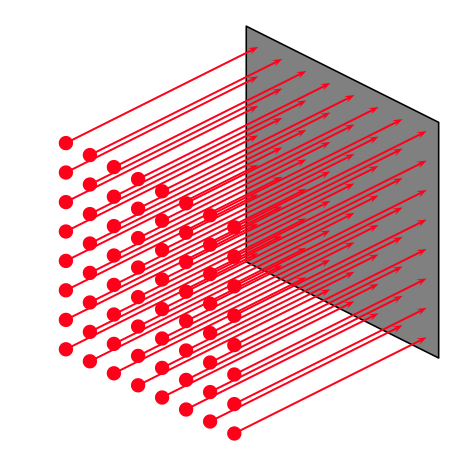
\includegraphics[scale=0.26]{parallelBeam}
& 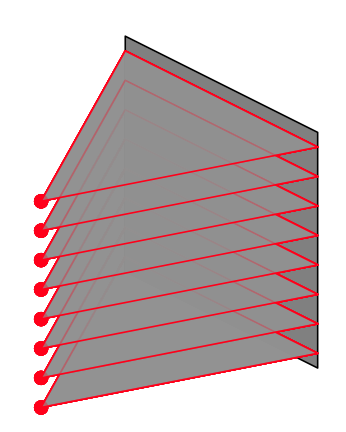
\includegraphics[scale=0.28]{fanBeam}
& 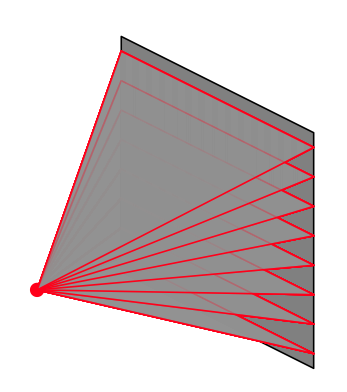
\includegraphics[scale=0.28]{coneBeam}
& 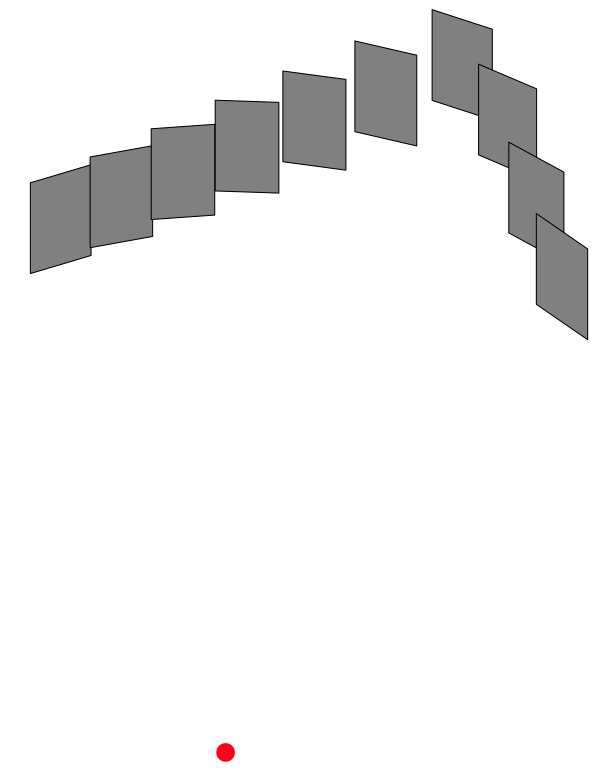
\includegraphics[scale=0.2]{modularBeam_cartoon}
\end{tabular}
\caption{Cartoon sketches of the parallel-, fan-, and cone-, and modular-beam geometries.} \label{fig:geometrySketches}
\end{figure}

We also provide projectors and analytic inversion algorithms, i.e., FBP, for a few specialized x-ray/Radon transforms:
\begin{enumerate}
\item Cylindrically-symmetric/anitsymmetric objects (related to the Abel Transform) in parallel- and cone-beam geometries with user-specified symmetry axis \cite{ChampleyMaddox_Optica_2021}. These are often used in flash radiography applications.
\item Attenuated Radon Transform (ART) for parallel-beam geometries. These are used in parallel-hole collimator SPECT and Volumetric Additive Manufacturing (VAM).
\end{enumerate}

In addition to the projectors, we also provide a few other algorithms for tomographic imaging, including:
\begin{enumerate}
\item Quantitatively-accurate analytic inversion algorithms, i.e., Filtered Backprojection (FBP) for each geometry including modular-beam when the detector columns are roughly align with the z-axis.
\item A GPU implementation of 3D anisotropic Total Variation (TV) functional, gradient, and quadratic form to be used in regularized reconstruction \cite{Yu_MIC_2006}.
\item Python implementations of some iterative reconstruction algorithms: MLEM, OSEM, OS-SART, ASD-POCS \cite{ASDPOCS_PMB_2008}, RWLS \cite{Hager_Zhang_CG_2005, Fessler_TIP_1999, Yu_MIC_2006}, RDLS, and ML-TR \cite{IMPACT_TMI_2001}.
\end{enumerate}

The CPU- and GPU-based projectors are nearly identical (32-bit floating point precision) and are quantitatively accurate and thus can be used in conjuction with physics-based corrections, such as, scatter and beam hardening correction. If one is looking for a more general-purpose and full functioning CT software package (it does not, however, work with PyTorch and is closed-source), see LTT \cite{ChampleyLTT}.

\section{Software Architecture}

There are three major layers in the architecture.  Users may interact with LEAP at any of these layers as each have their own API.  Each of these APIs is how we interact with it from a higher layer.  A diagram of the LEAP software architecture is shown in Figure \ref{fig:LEAParchitecture}.

\begin{figure}[h!]
\begin{center}
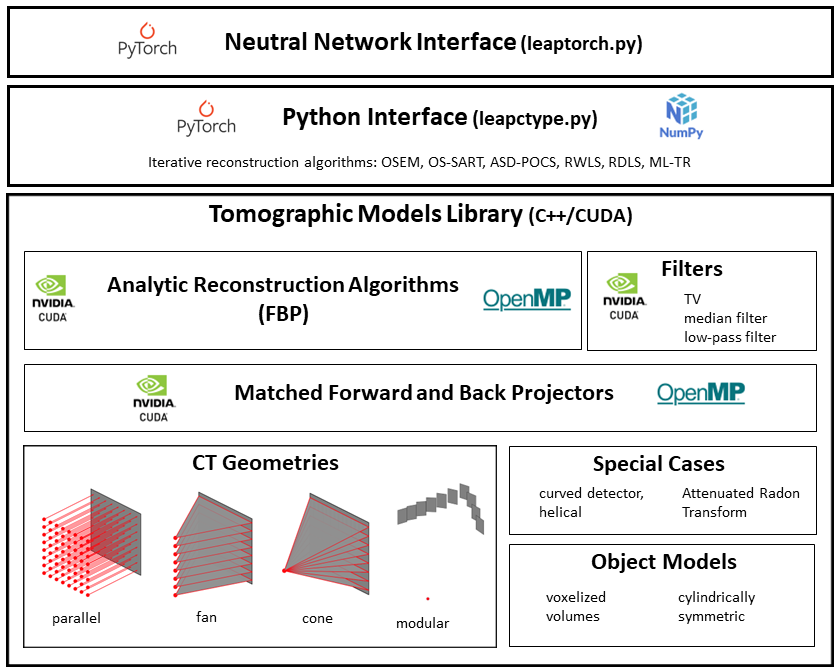
\includegraphics[scale=0.65]{LEAPoverview.png}
\end{center}
\vspace{-10pt}\caption{Overview of LEAP software architecture.} \label{fig:LEAParchitecture}
\end{figure}

The bottom C++/CUDA layer (Tomographic Models Library) contains all the forward projection, backprojection, FBP reconstruction, and imaging denoising algorithms.  This layer contains all the multi-GPU and multi-core CPU functionality.  This is the dynamic library (\textit{libleap.so} on Linux and \textit{libleap.dll} on Windows) that get compiled.  The main class is called \texttt{tomographicModels}.  All calls to LEAP must go through this class.  This class also contains a class called \textit{parameters} which contains all the CT geometry, CT volume parameters, and other run-time parameters.

The next layer is the primary Python interface, \textit{leapctype.py} (which is a Python class that is also called \texttt{tomographicModels}).  This provides an API to all the functionality in the bottom C++/CUDA layer and contains the iterative reconstruction algorithms.  If PyTorch is available it can take either PyTorch tensors or numpy arrays as input.  If PyTorch is not available, all the functionality still works.

The top layer provides the integration with the PyTorch neural network functionality using the \texttt{torch.nn.Module} and \texttt{torch.autograd.Function} PyTorch classes.  This code is contained in the file named \textit{leaptorch.py} which primarily consists of a class called \texttt{Projector}.  

The remainder of this document describes the algorithms in LEAP and the API class called \texttt{tomographicModels} which is in \textit{leapctype.py}.  Calls to this class can also be made from the \texttt{Projector} class in \textit{leaptorch.py} through the member variable named \texttt{leapct}.

\section{Troubleshooting Tools}

LEAP has a fair amount of parameters to specify and its algorithms are complex.  To assist users in troubleshooting, we have developed several tools.  The first tool simply prints all the parameter settings to the screen.  The function is given by
\begin{itemize}
    \item[] \texttt{print\_parameters()}.
\end{itemize}
The second tool builds a 3D sketch (using matplotlib) of the CT geometry and the CT volume.  This sketch can be generated by
\begin{itemize}
    \item[] \texttt{sketch\_system()}.
\end{itemize}
Example of the output of this function with a helical cone-beam geometry is shown in Figure \ref{fig:helicalSketch} and a modular-beam geometry is shown in Figure \ref{fig:modularBeamSketch}.

\begin{figure}[h!]
\begin{center}
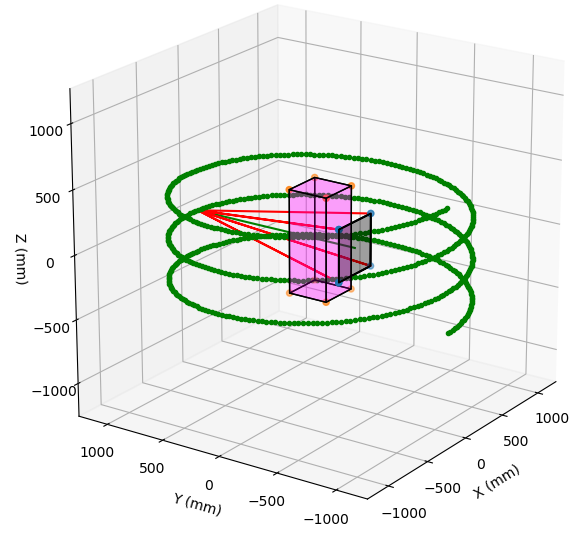
\includegraphics[scale=0.5]{helical}
\end{center}
\vspace{-20pt}\caption{Sketch of a helical cone-beam geometry generated with the \texttt{sketch\_system()} Python function.  The  magenta box is the reconstruction volume, the gray rectangle is the detector panel, the green dots are the source positions, and the red lines trace from the source to each of the four corners of the detector.} \label{fig:helicalSketch}
\end{figure}

The voxel locations of the specified volume can be retrieved by the \texttt{x\_samples()}, \texttt{y\_samples()}, and \texttt{z\_samples()} functions.  One can also use
\begin{itemize}
    \item[] \texttt{x,y,z = voxel\_samples()}
\end{itemize}
to get a 3D meshgrid of the samples.

\section{LEAP Parameters and General Syntax}

LEAP is a library of CT algorithms that operates on data arrays provided by the user.  These data arrays are the projection data and the volume data (see Section \ref{sec:dataArrays}).  The only permanent memory that LEAP manages itself is a class with member variables that parameterize the CT geometry and CT volume.  Some temporary memory is allocated during the computation of an algorithm but it is destroyed before the completion of the algorithm.  Prior to running any algorithm in LEAP, one must first set the CT geometry parameters and the CT volume parameters.

\subsection{Setting the CT Geometry Parameters}

Setting the CT geometry parameters is done by running one of the functions below
\begin{itemize}
\item[] \texttt{set\_parallelbeam(numAngles, numRows, numCols, pixelHeight, pixelWidth, centerRow, centerCol, phis)}
\item[] \texttt{set\_fanbeam(numAngles, numRows, numCols, pixelHeight, pixelWidth, centerRow, centerCol, phis, sod, sdd, tau=0.0)}
\item[] \texttt{set\_conebeam(numAngles, numRows, numCols, pixelHeight, pixelWidth, centerRow, centerCol, phis, sod, sdd, tau=0.0, helicalPitch=0.0)}
\item[] \texttt{set\_modularbeam(numAngles, numRows, numCols, pixelHeight, pixelWidth, sourcePositions, moduleCenters, rowVectors, colVectors)}
\end{itemize}
A description of these parameters can be found in Tables \ref{tab:stdGeometryParameters} and \ref{tab:modularParameters}.  The helical pitch is in units of mm/radian.  One can also set the normalized helical pitch (unitless) with the following function
\begin{itemize}
    \item[] \texttt{set\_normalizedHelicalPitch(normalized helical pitch)}.
\end{itemize}
The helical pitch, $\Delta$, and the normalized helical pitch $\widehat{\Delta}$ are related by
\begin{eqnarray*}
\widehat{\Delta} &:=& 2\pi \frac{\Delta}{\text{numRows} * \text{pixelHeight} * \frac{\text{sod}}{\text{sdd}}}.
\end{eqnarray*}

For cone-beam data, LEAP has implementations of both flat panel and curved panel setups.  See Section \ref{sec:conebeamTransform} for a description.  The default setting is flat panel, but one can switch between flat and curved panel detectors with the following commands
\begin{itemize}
\item[] \texttt{set\_flatDetector()}
\item[] \texttt{set\_curvedDetector()}.
\end{itemize}

\begin{table}[h!]
\caption{Parallel-, fan-, and cone-beam parameters.  Note that \texttt{sod}, \texttt{sdd}, and \texttt{tau} only apply to fan- and cone-beam geometries and \texttt{helicalPitch} only applies to cone-beam. The \texttt{centerRow} parameter has no effect on parallel- and fan-beam geometries.  Note that the \texttt{phis} parameter values \textit{must} be monotonic.  Internally, LEAP maintains a copy of the \texttt{phis} array, so if you want to make changes to it, you must either re-specify all parameters or use the \texttt{set\_angles()} function.  More information can be found in Section \ref{sec:CTGeometries}.} \label{tab:stdGeometryParameters}
\begin{tabular}{l|l|p{9cm}}
Parameter Name & Type & Description \\
\hline
\texttt{numAngles} & int32 & number of projection angles \\
\texttt{numRows} & int32 & number of detector rows \\
\texttt{numCols} & int32 & number of detector columns \\
\texttt{pixelHeight} & float32 & detector pixel pitch between rows (mm) \\
\texttt{pixelWidth} & float32 & detector pixel pitch between columns (mm) \\
\texttt{centerRow} & float32 & detector pixel row index for the ray that passes from the source, through the origin, and hits the detector \\
\texttt{centerCol} & float32 & detector pixel column index for the ray that passes from the source, through the origin, and hits the detector \\
\texttt{phis} & float32 array & array of the projection angles (degrees) \\
\texttt{sod} & float32 & source to object distance (mm) \\
\texttt{sdd} & float32 & source to detector distance (mm) \\
\texttt{tau} & float32 & horizontal translation of the rotation stage (mm) \\
\texttt{helicalPitch} & float32 & helical pitch (mm/radian)
\end{tabular}
\end{table}

\begin{table}[h!]
\caption{Modular-beam parameters.  Internally, LEAP maintains copies of \texttt{sourcePositions}, \texttt{moduleCenters}, \texttt{rowVectors}, and \texttt{colVectors}, so if you want to make changes to these, you must re-specify the modular-beam parameters.  More information can be found in Section \ref{sec:CTGeometries}.} \label{tab:modularParameters}
\begin{tabular}{l|l|p{9cm}}
Parameter Name & Type & Description \\
\hline
\texttt{numAngles} & int32 & number of projection angles \\
\texttt{numRows} & int32 & number of detector rows \\
\texttt{numCols} & int32 & number of detector columns \\
\texttt{pixelHeight} & float32 & detector pixel pitch between rows (mm) \\
\texttt{pixelWidth} & float32 & detector pixel pitch between columns (mm) \\
\texttt{sourcePositions} & float32 array & \texttt{numAngles} $\times$ 3 array of (x,y,z) coordinates of each source position \\
\texttt{moduleCenters} & float32 array & \texttt{numAngles} $\times$ 3 array of (x,y,z) coordinates of each detector center position \\
\texttt{rowVectors} & float32 array & \texttt{numAngles} $\times$ 3 array of vectors pointing in the positive detector row direction \\
\texttt{colVectors} & float32 array & \texttt{numAngles} $\times$ 3 array of vectors pointing in the positive detector row direction
\end{tabular}
\end{table}

To use the cylindrically-symmetric projectors, one must set the \texttt{axisOfSymmetry} parameter.  This is done using the following function
\begin{itemize}
    \item[] \texttt{set\_axisOfSymmetry(angleInDegrees)}
\end{itemize}
which must be a number between -30 and 30 degrees.  This axis of symmetry is nominally the z-axis.  The \texttt{axisOfSymmetry} parameter specifies the angle of rotation of the axis of symmetry around the x-axis.  One must specify \texttt{numAngles = 1} for this to work.

The Attenuated Radon Transform (ART) is used to model parallel-hole SPECT data and its adjoint can be used as a model in Volumetric Additive Manufacturing (VAM).  In  these contexts, the \textit{CT volume} in LEAP, plays the role as the activity concentration in units of Bq/mm$^3$.  To use the ART projectors, one must set the attenuation map and the CT geometry must be parallel-beam.  One can either specify this map as a voxelized volume (which must be defined on the same voxel grid as the standard volume and its units are in inverse length, e.g., mm$^{-1}$) or as a constant-valued function defined on a cylinder.  One can use the follow two functions to set this attenuation map.
\begin{itemize}
    \item[] \texttt{set\_attenuationMap(3D array)}
    \item[] \texttt{set\_cylindircalAttenuationMap(attenuationCoefficient, attenuationRadius)}
\end{itemize}
If using the second of these two functions, the \texttt{attenuationCoefficient} must be floating point number whose units are in inverse length (e.g., mm$^{-1}$) and the \texttt{attenuationRadius} must be a floating point number listed in length units (e.g., mm).  Only GPU projectors are defined for the arbitrary attenuation map.  The constant-valued attenuation map work for both CPU and GPU processing and is much faster.  Analytic inversion algorithms are carried out via Novikov's formula \cite{Natterer_IP_2001} and must have at least 360 degrees of angular coverage.  For a mathematical description of this transform, see Section \ref{sec:ART}.

\subsection{Setting the CT Volume Parameters}

Next, the user should specify the CT volume parameters.  This can be done in one of the two following ways:
\begin{itemize}
\item[] \texttt{set\_volume(numX, numY, numZ, voxelWidth, voxelHeight, offsetX, offsetY, offsetZ)}
\item[] \texttt{set\_default\_volume()}
\end{itemize}
Using the \texttt{set\_default\_volume()} function (after the CT geometry parameters are set) sets the CT volume parameters to fill the field of view of the CT system with the nominal voxel sizes.  A description of these parameters can be found in Table \ref{tab:volumeParameters}.

\begin{table}[h!]
\caption{CT volume parameters.  A full description of these parameters can be found in Section \ref{sec:VolumeParameterization}.} \label{tab:volumeParameters}
\begin{tabular}{l|l|p{9cm}}
Parameter Name & Type & Description \\
\hline
\texttt{numX} & int32 & number of voxels in the x-dimension \\
\texttt{numY} & int32 & number of voxels in the y-dimension \\
\texttt{numZ} & int32 & number of voxels in the z-dimension \\
\texttt{voxelWidth} & float32 & voxel pitch (size) in the x and y dimensions (mm) \\
\texttt{voxelHeight} & float32 & voxel pitch (size) in the z dimension (mm) \\
\texttt{offsetX} & float32 & shift the volume in the x-dimension (mm) \\
\texttt{offsetY} & float32 & shift the volume in the y-dimension (mm) \\
\texttt{offsetZ} & float32 & shift the volume in the z-dimension (mm)
\end{tabular}
\end{table}

\subsection{Layout of the Data Arrays} \label{sec:dataArrays}

The data arrays must be contiguous.  The order of the projection data indices is listed as follows
\begin{itemize}
\item[] \texttt{projection\_data[iAngle*numRows*numCols + iRow*numCols + iCol]},
\end{itemize}
where iAngle, iRow, and iCol are the indices of the angle, row, and column dimensions.  The volume data can be in ZYX or XYZ order.  The ZYX order is the default setting.  To switch to the XYZ ordering do: \texttt{set\_volumeDimensionOrder(0)}.  The ZYX ordering works best for GPU processing (and is \textit{required} for multi-GPU processing) and the XYZ ordering works best for CPU processing.  To be clear the ZYX ordering is as follows
\begin{itemize}
\item[] \texttt{volume\_data[iZ*numY*numX + iY*numX + iX]}
\end{itemize}
and the XYZ ordering is as follows
\begin{itemize}
\item[] \texttt{volume\_data[iX*numY*numZ + iY*numZ + iZ]},
\end{itemize}
where iX, iY, and iZ are the indices of the x, y, and z dimensions.  To help assist users in allocating contiguous arrays in the correct order in Python we provide the follow Python functions
\begin{itemize}
    \item[] \texttt{allocateProjections()}
    \item[] \texttt{allocateVolume()}
\end{itemize}

\section{CPU/GPU Processing}

As stated above, the algorithm in LEAP are written for both multi-GPU and multi-core CPU processing.  If one has at least one GPU, then GPU is the default processing.

There is an integer array parameter in LEAP where you specify which GPUs you would like to use.  This parameter can be set with the function
\begin{itemize}
\item[] \texttt{set\_GPUs(list of integers)}.
\end{itemize}
GPUs are listed on a computer as integers start at zero.  The first number in this list is considered the primary GPU.  For small computations it is advantageous to only use one GPU and not transfer any data on/off this GPU.  Thus if the data is already on the GPU, LEAP will only use this GPU for processing.  On the other hand, if the data is on the CPU memory, then the data will be transferred to each GPU in your list, the computation is carried out and then the result is copied back to the CPU array you specified.

For convenience, we also provide the function: \texttt{set\_GPU(gpu index)} to only set a single GPU.  To switch to CPU processing, run this command: \texttt{set\_GPU(-1)}.

\section{A Note on Coordinate Systems}

LEAP uses the standard right-hand coordinate system, but there are important subtleties in CT coordinate systems so we thought we'd start off by describing these.  Typical two-dimensional Cartesian coordinate systems have the positive x-coordinate pointing to the right and the positive y-coordinate pointing up.  On the other hand, typical digital image coordinates have the column coordinate pointing to the right and the row coordinate pointing \textit{down}.  This discrepancy between digital image coordinates and Cartesian coordinates causes endless confusion.  Images are displaced on a computer screen this way and digital x-ray detectors record data this way as well.  Thus, in LEAP, we make the effort to use the digital image coordinate system as well as we can.

Thus, we define detector coordinates as digital image coordinates with the origin at the top-left side of the image/detector.  So that out Cartesian coordinates more closely match this convention, our z-axis shall be parallel to the detector row coordinate (and point in the same direction) and our x-axis shall be parallel to the detector column coordinate (and point in the same direction).  The y-axis shall be oriented to make a right-hand coordinate system.  A sketch of these coordinates in the cone-beam geometry is shown in Figure \ref{fig:coneBeamSketch}.

\begin{figure}[h]

%\begin{figure}[h]
\psset{unit=0.15mm,linewidth=1.5pt,drawCoor=false,Alpha=55}
\pspicture(-600,-425)(200,250)%

\pstThreeDLine(-173.16, 400, -248.03)(256.72, 400, -248.03)(256.72, 400, 182.38)(-173.16, 400, 182.38)(-173.16, 400, -248.03) % outline of detector
%\pstThreeDDot(85.44, -593.89, 0) % dot at source position
\pstThreeDDot(0.0, -600.0, 0) % dot at source position
\pstThreeDDot[linewidth=3pt,linecolor=red](0,0,0) % dot at origin
\pstThreeDLine[linewidth=3pt]{->}(-173.16, 400, 182.38)(-173.16, 400, 82.378) % v vector
\pstThreeDLine[linewidth=3pt]{->}(-173.16, 400, 182.38)(-73.158, 400, 182.38) % u vector
%\pstThreeDLine(85.44, -593.89, 0)(85.44, 400, 0) % line to perp
%\pstThreeDLine(85.44, -593.89, 0)(0,0,0)(-43.16, 400, 0) % line to pxcenter
\pstThreeDLine(0.0, -600.0, 0)(0.0, 400, 0) % line to perp
\pstThreeDLine(0.0, -600.0, 0)(0,0,0)(0.0, 400, 0) % line to pxcenter
%\pstThreeDLine[linestyle=dotted](-43.16, 400, -248.03)(-43.16, 400, 182.38) % pxcenter column
\pstThreeDLine[linestyle=dotted](-0.0, 400, -248.03)(-0.0, 400, 182.38) % pxcenter column
%\pstThreeDLine[linestyle=solid]{->}(85.44, 400, -98.034)(-43.16, 400, -98.034)
%\pstThreeDLine[linestyle=dotted](85.44, 400, -248.03)(85.44, 400, 182.38) % pxoffset column
%\pstThreeDLine[linestyle=solid]{->}(-173.16, 400, -173.03)(85.44, 400, -173.03) % s_c arrow
\pstThreeDLine[linestyle=solid]{->}(-173.16, 400, -120.03)(0.0, 400, -120.03) % s_c arrow
%\pstThreeDLine(135.44, 400, 0)(135.44, 350, 0)(85.44, 350, 0) % perp
\pstThreeDLine[linestyle=dotted](-173.16, 400, 0)(256.72, 400, 0) % pzcenter column
\pstThreeDLine[linestyle=solid]{->}(-123.16, 400, 182.38)(-123.16, 400, 0) % pzcenter arrow

% detector labels
\pstThreeDPut(-200,400,80){\Large $j$}
\pstThreeDPut(-90,400,220){\Large $i$}
\pstThreeDPut(-50,400,-160){\Large $i_c$}
\pstThreeDPut(-90,400,70){\Large $j_c$}
%\pstThreeDPut(0,400,-130){\Large $s_0$}

\pstThreeDPut(80,-600,20){\Large source}
%\pstThreeDPut(80,-630,-50){\large (0,sod,0)}
%\pstThreeDPut(0,0,31){\Large center of rotation/origin}
%\pstThreeDPut(-160,400,-60){\large (0,odd,0)}

\pstThreeDLine[linestyle=dashed]{<->}(-50,-600,0)(-50,0,0)
\pstThreeDPut(-100,-300,0){\Large sod}
\pstThreeDLine[linestyle=dashed]{<->}(100,-600,0)(100,400,0)
\pstThreeDPut(140,-300,0){\Large sdd}

\pstPlanePut[plane=xz,planecorr=normal](90,400,-290){\Large detector}

%\pstThreeDCoor[xMin=-150,xMax=150,yMin=150,yMax=-150,zMin=150,zMax=-150]
\pstThreeDLine[linestyle=solid,linecolor=red]{->}(-150,0,0)(150,0,0)
\pstThreeDLine[linestyle=solid,linecolor=red]{->}(0,150,0)(0,-150,0)
\pstThreeDLine[linestyle=solid,linecolor=red]{->}(0,0,150)(0,0,-150)
\pstThreeDPut(150,0,-20){\Large x}
\pstThreeDPut(0,-150,-30){\Large y}
\pstThreeDPut(-30,0,-150){\Large z}

\endpspicture

\caption{LEAP provides forward and backprojectors and FBP reconstruction algorithms for a flexible cone-beam geometry.  Note that $(i,j)$ are detector column and row index coordinates, respectively, and \texttt{i\_c = centerCol} and \texttt{j\_c = centerRow}.} \label{fig:coneBeamSketch}
\end{figure}

\section{CT Geometries} \label{sec:CTGeometries}

In this section we discuss the parameterization of the four LEAP scanner geometry types: parallel-, fan-, cone-, and modular-beam.  Cartoon sketches of the parallel-, fan-, cone-, and modular-beam geometries is shown in Figure \ref{fig:geometrySketches} and a detailed sketch of the cone-beam coordinates in Figure \ref{fig:coneBeamSketch}.  We also give the mathematical expressions that link sets of parameterizations, state conjugate ray expressions, and the adjoint of the forward projection operators which are often referred to as backprojection operators.  Unless otherwise stated, all LEAP algorithms can be applied to any scanner geometry type.  This feature is made possible by the fact that data for all geometry types can be stored in contiguous 3D arrays (view number, detector row, detector column) and that most of the differences can be encapsulated in the implementation of the forward and back projectors.  Two-dimensional geometries can be achieved by setting the number of detector rows and number of z-slices to one.

\subsection{Detector Coordinates} \label{sec:DetectorCoordinates}

We denote detector coordinates by $(s,t)$.  The center position of the pixel coordinates are given by the following equations:
\begin{eqnarray*}
s[i] &=& \text{pixelWidth}*(i - \text{centerCol}), \text{ for } i = 0, \dots, \text{numCols}-1, \\
t[j] &=& \text{pixelHeight}*(j - \text{centerRow}), \text{ for } j = 0, \dots, \text{numRows}-1,
\end{eqnarray*}
where pixelWidth and pixelHeight are assumed to be in length units, e.g., mm or cm.  The indicies of the center detector column and center detector row are given by centerCol and centerRow, respectively.  For a perfectly centered detector, $\text{centerCol} = 0.5(\text{numCols}-1)$ and $\text{centerRow} = 0.5(\text{numRows}-1)$.

\subsection{Volume Parameterization} \label{sec:VolumeParameterization}

The location of the 3D voxels are specified by seven parameters as follows
\begin{eqnarray*}
x[i] &=& \text{voxelWidth}*(i - 0.5*(\text{numX}-1)) + \text{offsetX}, \text{ for } i = 0, \dots, \text{numX}-1, \\
y[j] &=& \text{voxelWidth}*(j - 0.5*(\text{numY}-1)) + \text{offsetY}, \text{ for } j = 0, \dots, \text{numY}-1, \\
z[k] &=& \text{voxelHeight}*(k - 0.5*(\text{numZ}-1)) + \text{offsetZ}, \text{ for } k = 0, \dots, \text{numZ}-1
\end{eqnarray*}
Here, voxelWidth, voxelHeight, offsetX, offsetY, and offsetZ are assumed to be in length units, e.g., mm or cm.  Make sure that whatever units of length you choose that you stay consistent across all parameters.  The units of the voxelized volume (i.e., the reconstruction volume) are assumed to be in inverse length, e.g., mm$^{-1}$ or cm$^{-1}$.  We make this distinction because LEAP is fairly unique in it's quantitatively-accurate algorithms which we believe is very useful.

As a reminder, one can be the \texttt{x\_samples()}, \texttt{y\_samples()}, and \texttt{z\_samples()} functions to retrieve numpy arrays of the volume coordinate loctions.

We note that there are some restrictions in the above volume parameters based on the CT geometry one is using.  These restrictions are listed below.
\begin{itemize}
\item parallel-beam
    \begin{itemize}
    \item voxelHeight must be equal to pixelHeight
    \item offsetZ must be zero
    \item numZ must be equal to numRows
    \end{itemize}
\item fan-beam
    \begin{itemize}
    \item voxelHeight must be equal to pixelHeight
    \item offsetZ must be zero
    \item numZ must be equal to numRows
    \end{itemize}
\item cone-beam
    \begin{itemize}
    \item no restrictions
    \end{itemize}
\item modular-beam, when rowVectors is approximately equal to the z-axis
    \begin{itemize}
    \item no restrictions
    \end{itemize}
\item modular-beam, when rowVectors is not approximately equal to the z-axis
    \begin{itemize}
    \item voxelHeight must be equal to voxelWidth
    \end{itemize}
\end{itemize}
The restrictions for parallel- and fan-beam are that there is a one-to-one correspondence between the volume z-slices and the detector rows.  If any of the above restrictions are violated, then LEAP will return an error when a forward projection, backprojection, or FBP algorithm is called.

Besides the above restrictions, there are recommended values for the voxel sizes.  If the voxel size is significantly smaller or significantly bigger than these recommended sizes, then the LEAP algorithms may run much, much slower.

\begin{itemize}
\item parallel-beam
    \begin{itemize}
    \item recommend that voxelWidth be equal to pixelWidth
    \end{itemize}
\item fan-beam
    \begin{itemize}
    \item recommend that voxelWidth be equal to pixelWidth*sod/sdd
    \end{itemize}
\item cone-beam
    \begin{itemize}
    \item recommend that voxelWidth be equal to pixelWidth*sod/sdd
    \item recommend that voxelHeight be equal to pixelHeight*sod/sdd
    \end{itemize}
\item modular-beam
    \begin{itemize}
    \item recommend that voxelWidth be equal to pixelWidth/2
    \end{itemize}
\end{itemize}

It is recommended that one specify the volume parameters with the set\_default\_volume() command which sets the volume to fill the field of view of the CT system and use the recommended voxel sizes.

Note that the voxel samples are aligned with the x,y,and z axes and there are no methods to rotate these coordinates.  This restriction is for a few reasons.  First of all, there are certain rotations that are incompatible with Separable Footprint projectors.  Second, there are certain assumptions that one can leverage with standard CT geometry types (parallel, fan, and cone) that improve the computational efficiency of the projectors.  In fact, the complexity of the CT geometry is highly related to the computation speed of it projectors.  The speed of the projectors, listed from fasted to slowest, is: parallel-, fan-, cone-, and modular-beam.  And finally, it is easier to subdivide the volume into smaller chunk to process operations across multiple GPUs or to split it up into chunks that can fit into the GPU memory.  All of that being said, there are two \textit{tricks} to perform some rotations of the voxel coordinates.  First, for modular-beam coordinates, one may simply perform the inverse rotation on the location and orientation of the source locations and detector locations and orientations that will effectively rotate the volume coordinates.  Second, one may provide a phase shift of the provided projection angles which effectively rotates the volume coordinates around the z-axis.  Lastly, one may utilize the offsetX, offsetY, and offsetZ parameters to perform projections and backprojections of a single 2D plane or a single voxel at a time to generate a custom voxel grid.  This scheme, however, is less efficient and more difficult to manage.

In the next section we describe the integral transforms and inversion algorithms for parallel-, fan-, and cone-beam geometries.

\subsection{X-ray Transform and Its Adjoint}

Consider a linear operator denoted by $\mathcal{A}$.  Then its adjoint, usually denoted by $\mathcal{A}^*$, is defined such that $$<\mathcal{A}x, y> = <x, \mathcal{A}^*y>.$$  Note that if $\mathcal{A}$ where a real-valued matrix, its adjoint would be equal to its transpose.

The X-ray Transform of $f \in L^1(\mathbb{R}^3)$ is a linear operator given by
\begin{eqnarray*}
    Pf(\B{y}, \Theta) = \int_\mathbb{R} f(\B{y} + l\Theta) \, dl,
\end{eqnarray*}
where in general $y, \Theta \in \mathbb{R}^3$, but the exact specification of these parameters depends on the geometry of the CT system.  The X-ray Transform is often referred to as a \textit{projection} or \textit{forward projection} of a function.  While the adjoint of the X-ray Transform is commonly referred to as the \textit{backprojection} operator.  The backprojection operator usually takes the form of an integral over the various measured angles of the X-ray transform, but its exact form depends on the parameterization of the line integrals in the forward projection.

In the following, we shall make use of the following definitions
\begin{eqnarray*}
\theta &:=& \theta(\varphi) := \begin{bmatrix} \cos\varphi \\ \sin\varphi \\ 0 \end{bmatrix} \\
\theta^\perp &:=& \theta^\perp(\varphi) := \begin{bmatrix} -\sin\varphi \\ \cos\varphi \\ 0 \end{bmatrix}.
\end{eqnarray*}
We shall usually denote $g = Pf$.

\subsection{Parallel-Beam}

The X-ray transform and its adjoint in parallel-beam coordinates are given by 
\begin{eqnarray*}
Pf(s, \varphi, x_3) &:=& \int_\mathbb{R} f(s\bm{\theta}^\perp(\varphi) - l\bm{\theta}(\varphi) + x_3\B{e}_3) \, dl \\
P^*g(\bm{x}) &=& \int_0^{2\pi} g(\bm{x}\cdot\bm{\theta}^\perp(\varphi), \varphi, x_3) \, d\varphi
\end{eqnarray*}
Note that $g(s,\varphi) = g(-s,\varphi \pm \pi)$; the rays defined by these two coordinates are known are conjugate rays.

The object, $f$, can be reconstructed by
\begin{eqnarray*}
f(\bm{x}) &=& \frac{1}{4\pi} \int_0^{2\pi} \int_\mathbb{R} h(\bm{x}\cdot\bm{\theta}^\perp(\varphi) - s) g(s,\varphi, x_3) \, ds \, d\varphi.
\end{eqnarray*}
The discretization of the above equation is referred to as filtered backprojection (FBP).  The function $h$ is referred to as the ramp filter and is described in Section \ref{sec:rampFilter}.

% arctan(2*t*R/(R^2-t^2)) = 2*arcsin(t/sqrt(R^2+t^2))
\subsection{Fan-Beam}

\begin{comment}
\begin{figure}[h] % 626.5664, 1026.5664
\begin{center}
\psset{unit=1.1mm}
\begin{pspicture}(-60,-60)(63,65)
\psline[linewidth=1.25pt]{<->}(0,70)(0,0)(70,0)
\pscircle[linestyle=dashed](0,0){62.8558} \rput{90}(-62,0){\parbox{2.1 cm}{\large \B{source trajectory}}} % source trajectory
\rput{-22}(19,17){$R\bm{\theta}-l[\bm{\theta}$} % X-ray trajectory
\qdisk(-47.8405, 40.7694){3.5 pt} \rput(-50,45){\Large R$\bm{\theta}$} % source
%\psarc{->}(0, 0){65}{141}{150} % source trajectory
\psline[linestyle=dotted](-47.8405, 40.7694)(-3.5355,-3.5355)(21.2487,-28.3198) % line from source to detector
%\psline(21.9203, -28.9914)(19.0918, -31.8198)(21.9203, -34.6482) % perpendicular on detector
\psline[linestyle=dashed](-3.5355,-3.5355)(20,-3.5355) % line for angle start
\rput(-23,12){\Large $R$} % R
\rput(-0.5,-15){\Large $D-R$} % D
\psline[linestyle=dashed](-47.8405, 40.7694)(49.3427, 1.3120) % LOR
%\psarc[linewidth=1.5pt]{->}(-47.8405, 40.7694){102.65664}{-69}{-20} \rput{45}(26.4645,-33.5355){\large \B{detector}} \rput(50, 8){\Large $i$} % detector
\psline(-10,-60)(60, 10)
%\pscircle[linestyle=dotted](0,0){25} % FOV
\psarc[linecolor=blue]{->}(-3.5355,-3.5355){10}{0}{135} \rput(-5,9){\blue \Large $\beta$} % beta
\psarc[linecolor=blue]{->}(-47.8405, 40.7694){20}{-45}{-22} \rput(-29,28){\blue \Large $\alpha$} % alpha
\psline[linecolor=red](-3.5355,-3.5355)(7.2046, 18.4849) \rput(3.8,9.0){\red \Large $s$} % s
%\psarc[linecolor=red]{->}(-3.5355,-3.5355){18}{0}{64} \rput(13,8){\red \Large $\varphi$} % phi
%\psline(7.3366, 18.1587)(2.7969, 19.9929)(4.6311, 24.5326)
\psline(5.2319,14.4403)(0.7379,16.6322)(2.6010, 20.4521)
\qdisk(0,0){2.5pt} % center of rotation; origin
\psset{linecolor=aclr}\qdisk(-3.5355,-3.5355){2 pt}\psset{linecolor=black} % iso-center
\psline[linecolor=aclr,linewidth=1.5pt](0,0)(-3.5355,-3.5355) \rput(-0.25,-2.75){\Large \color{aclr} $\tau$} % tau
%\psline{<->}[linestyle=dashed](-53.8405, 34.7694)(18.7487,-37.8198) \rput(-13,-10){\Large $D$} % D
\rput(70,-3){\Large $x_1$} \rput(-3,68){\Large $x_2$}
\end{pspicture}
\caption{Fan-beam coordinates and their relation to parallel beam coordinates.  Note that the isocenter is indicated by a turquoise dot and the center of rotation is indicated by a black dot and is located at the origin.} \label{fig:fanBeam}
\end{center}
\end{figure}
\end{comment}

The X-ray transform and its adjoint in fan-beam coordinates (with linear detector) with center of rotation offset of $\tau$, source to object distance (sod) $R$, and source to detector distance $D$, are given by
\begin{eqnarray*}
Pf(u,\beta,x_3) &:=& \int_\mathbb{R} f\left(R\bm{\theta}(\beta) - \tau\bm{\theta}^\perp(\beta) - \frac{l}{\sqrt{1+u^2}}\left[\bm{\theta}(\beta) - u\bm{\theta}^\perp(\beta) \right] + x_3\B{e}_3 \right) \, dl \\
P^*g(\bm{x}) &=& \int \frac{1}{R-\bm{x}\cdot\bm{\theta}(\beta)} \sqrt{1 + u^2(\bm{x},\beta)} g\left( u(\bm{x},\beta), \beta, x_3\right) \, d\beta \\
u(\bm{x},\beta) &:=& \frac{\bm{x}\cdot \bm{\theta}^\perp(\beta) + \tau}{R - \bm{x}\cdot\bm{\theta}(\beta)}
\end{eqnarray*}
The parameter $u$ is the detector column coordinate divided by sdd and can be viewed as the slope of the ray in the xy plane.  Note the conjugate ray relation is $$g(u,\beta,x_3) = g\left(\frac{-u+\frac{2\tau R}{R^2-\tau^2} }{1 + u\left(\frac{2\tau R}{R^2-\tau^2}\right)}, \beta-2\tan^{-1}u + \tan^{-1}\left(\frac{2\tau R}{R^2-\tau^2}\right) \pm \pi, x_3 \right).$$

The object, $f$, can be reconstructed by the following Filtered Backprojection (FBP) algorithm
\begin{eqnarray*}
f(\bm{x}) &=& \frac{R}{2\pi} \int \frac{1}{(R-\bm{x}\cdot\bm{\theta}(\beta))^2} \int_\mathbb{R} h\left( u(\bm{x},\beta) - u \right) g(u, \beta, x_3) m(\tan^{-1}u,\beta) \frac{1 + \frac{\tau}{R}u}{\sqrt{1+u^2}} \, du \, d\beta.
\end{eqnarray*}
The function $m$ accounts for the number of redundant measurements for a particular angle and for an angular range of less than 360$^\circ$ it is often referred to as the \textit{Parker Weights}; See Section \ref{sec:ParkerWeighting}.  The function $h$ is referred to as the ramp filter and is described in Section \ref{sec:rampFilter}.

%\tan^{-1}\left(\frac{2\tau R}{R^2-\tau^2}\right)

Parallel-beam and fan-beam coordinates are related by the following transformations:
\begin{eqnarray*}
s &=& \frac{Ru-\tau}{\sqrt{1+u^2}}, \\
\varphi &=& \beta - \tan^{-1}u %\\
%\alpha &=& \tan^{-1}u.
\end{eqnarray*}
%where $R_{\tau} = \sqrt{R^2+\tau^2}$.

%Typically $R$ is referred to as the source-to-object distance (sod), $R_{\tau}$ is referred to as the source-to-object distance (sod), and $D$ is referred to as the source-to-detector distance (sdd).

%Let $i$ be the detector coordinate.  Then $u = \frac{i}{D}$ and $\alpha = \tan^{-1}\left(\frac{i}{D}\right)$.

\subsection{Cone-Beam} \label{sec:conebeamTransform}

The X-ray transform and its adjoint in cone-beam coordinates (with planar detector) with center of rotation offset of $\tau$, source trajectory radius $R$, and helical pitch $\Delta$ are given by
\begin{eqnarray*}
Pf(u,\beta,v) &:=& \int_\mathbb{R} f\left(R\bm{\theta}(\beta) - \tau\bm{\theta}^\perp(\beta) + \Delta\varphi\widehat{\bm{z}}  + \frac{l}{\sqrt{1+u^2+v^2}}\left[-\bm{\theta}(\beta)+u\bm{\theta}^\perp(\beta) + v\widehat{\bm{z}} \right] \right) \, dl \\
P^*g(\bm{x}) &=& \int \frac{\sqrt{1+ u^2(\bm{x},\beta) +v^2(\bm{x},\beta)}}{(R-\bm{x}\cdot\bm{\theta}(\beta))^2} g\left( u(\bm{x},\beta), \beta, v(\bm{x},\beta)\right) \, d\beta \\
u(\bm{x},\beta) &:=& \frac{\bm{x}\cdot \bm{\theta}^\perp(\beta) + \tau}{R - \bm{x}\cdot\bm{\theta}(\beta)} \\
v(\bm{x},\beta) &:=& \frac{x_3 - \Delta\varphi}{R - \bm{x}\cdot\bm{\theta}(\beta)}
\end{eqnarray*}
The parameter $v$ is the detector row coordinate divided by sdd and can be viewed as the slope of the ray.

When $\Delta = 0$ (axial scan), the object, $f$, can be (approximately) reconstructed with the Feldkamp, Davis, and Kress (FDK) algorithm \cite{FDK} which is a type of Filtered Backprojection (FBP) algorithm
\begin{eqnarray*}
f(\bm{x}) &\approx& \frac{R}{2\pi} \int \frac{1}{(R-\bm{x}\cdot\bm{\theta}(\beta))^2} \\ &\times& \int_\mathbb{R} h(u(\bm{x},\beta) - u) g(u,\beta, v(\bm{x},\beta)) m(\tan^{-1}u,\beta) \frac{1+\frac{\tau}{R}u}{\sqrt{1+u^2+v^2(\bm{x},\beta)}} \, du \, d\beta.
\end{eqnarray*}
The function $h$ is referred to as the ramp filter and is described in Section \ref{sec:rampFilter}.

X-ray CT systems commonly used in medical and security applications employ a curved detector that approximately fits the surface of a cylinder whose center is at the x-ray source.  In this setup, we have the \textit{curved} cone-beam coordinates.  The X-ray transform and its adjoint in curved cone beam coordinates with center of rotation offset of $\tau$ and source trajectory radius $R$ are given by
\begin{eqnarray*}
Pf(\alpha,\beta,\nu) &=& \int_\mathbb{R} f\left(R\bm{\theta}(\beta) - \tau\bm{\theta}^\perp(\beta) + \Delta\varphi\widehat{\bm{z}} + \frac{l}{\sqrt{1+\nu^2}}\left[-\bm{\theta}(\beta-\alpha) + \nu\widehat{\bm{z}} \right] \right) \, dl \\
P^*g(\bm{x}) &=& \int \frac{\sqrt{1+\nu^2(\bm{x},\beta)}}{\| R\bm{\theta}(\beta) - \tau\bm{\theta}^\perp(\beta) - \bm{x} \|^2}  g\left(\alpha(\bm{x},\beta), \beta, \nu(\bm{x},\beta)\right) \, d\beta \\
\alpha(\bm{x},\beta) &:=& \tan^{-1}\left( \frac{\bm{x}\cdot \bm{\theta}^\perp(\beta) + \tau}{R - \bm{x}\cdot\bm{\theta}(\beta)} \right) \\
\nu(\bm{x},\beta) &:=& \frac{x_3 - \Delta\varphi}{\|R\bm{\theta}(\beta) - \tau\bm{\theta}^\perp(\beta) - \bm{x} \|}
\end{eqnarray*}
Note that the $v$ and $\nu$ are related by $v = \sqrt{1+u^2}\nu$ and $u$ and $\alpha$ are related by $u = \tan\alpha$.

When $\Delta = 0$ (axial scan) the object, $f$, can be approximately reconstructed by
\begin{eqnarray*}
f(\bm{x}) &\approx& \frac{R}{2\pi} \int \frac{1}{\| R\bm{\theta}(\beta) - \tau\bm{\theta}^\perp(\beta) - \bm{x} \|^2} \\ &\times& \int_{-\pi/2}^{\pi/2} h(\sin(\alpha(\bm{x},\beta) - \alpha)) g(\alpha, \beta, \nu(x,\beta)) m(\alpha, \beta) \frac{\left(\cos\alpha + \frac{\tau}{R}\sin\alpha\right)}{\sqrt{1+\nu^2(\bm{x},\beta)}} \, d\alpha \, d\beta.
\end{eqnarray*}

Although theoretically-exact reconstruction of helical cone-beam data can be acheived with the Katsevich algorithm \cite{Katsevich_SIAM_2002}, this algorithm is not able to use all the measured data and produces artifacts when the number of contributions to portions of the frequency-space of the reconstruction has an abrupt transition.  For this reason we chose to implement a variation of the WFBP \cite{WFBP} algorithm.  This algorithm was derived in \textit{cone-parallel} coordinates, so we re-derived this algorithm for the native cone-beam coordinates.  The view derivative step of the algorithm was implemented by the NHDLH \cite{NHDLH_PMB_2007} method which provides good resolution across the imaging field of view.

We would like to take a special note in the exact form of the adjoint of the cone-beam X-ray Transform.  Notice that
\begin{eqnarray*}
P^*g(\B{x}) &\neq& \int_\mathbb{R} g(u(\B{x},\beta), \beta, v(\B{x},\beta)) \, d\beta.
\end{eqnarray*}
The right hand side of the above equation is what many say is the backprojection operator, but this is false.  A backprojection is not always merely an integral over all the measured angles for those rays going through a specific point in space.  Thus it is also often said that FBP reconstruction of cone-beam data requires a \textit{weighted} backprojection because of the $\frac{1}{R-\B{x}\cdot\theta}$ term, but we see that this term is actually present in the backprojection already.  This origin of this term is the Jacobian of the change of coordinates matrix when deriving the backprojection.  One of the nice things about using match projector pairs, is that this weighting term is implicitly included when performing the backprojection operation.

\subsection{Parker Weighting} \label{sec:ParkerWeighting}

This section defines the so-called \textit{Parker Weights} \cite{Parker_MP_1982} which enable reconstruction of a \textit{short-scan} of fan- or cone-beam data.  A \textit{short-scan} is defined as a scan that acquires at least 180 plus the fan angle, but less than 360 degrees of projection angles. Define $\alpha := \tan^{-1}(u)$.  The function $m(\cdot, \cdot)$ given above is known as the Parker weighting function.  For a short scan, where $\pi + 2\alpha_{max} + \tan^{-1}\left(\frac{2\tau R}{R^2-\tau^2}\right) \leq \beta_{end}-\beta_0 < 2\pi$, it is given by
\begin{eqnarray*}
m(\alpha, \beta) &:=& \begin{cases} \sin^2\left( \frac{\pi}{4} \frac{\beta-\beta_0}{\alpha_{thres} - \alpha} \right), & 0 \leq \beta-\beta_0 < 2(\alpha_{thres}-\alpha), \\ 1, & 2(\alpha_{thres} - \alpha) \leq \beta-\beta_0 < \pi - 2\alpha - \tan^{-1}\left(\frac{2\tau R}{R^2-\tau^2}\right), \\ \cos^2\left( \frac{\pi}{4} \frac{(\beta-\beta_0) + 2\alpha + \tan^{-1}\left(\frac{2\tau R}{R^2-\tau^2}\right) - \pi}{\alpha_{thres}+\alpha} \right), & \pi-2\alpha-\tan^{-1}\left(\frac{2\tau R}{R^2-\tau^2}\right) \leq \beta-\beta_0 < \pi + 2\alpha_{thres}, \end{cases}
\end{eqnarray*}
where $\alpha_{thres} = \frac{\beta_{end}-\beta_0 - \pi}{2}$.  For a full scan, i.e., when $\beta_{end}-\beta_0 = 2\pi$, we have $m(\alpha, \beta) = \frac{1}{2}$.

%\begin{comment}
One may increase the transaxial field of view \cite{Gullberg_TMI_1986, Gregor_ICI_2003} by shifting the detector to one side or by deliberately giving the center of rotation a large offset, i.e.., $|\tau| \gg 0$; see Figure \ref{fig:offsetScan}.  In this case one must acquire a full scan.  See Figure \ref{fig:offsetScan}.  First we let
\begin{eqnarray*}
\delta_{min} &=& \left| R\sin\alpha_{min}-\tau \cos\alpha_{min}\right| \\
\delta_{max} &=& \left| R\sin\alpha_{max}-\tau \cos\alpha_{max}\right|.
\end{eqnarray*}
Then if $\delta_{min} < \delta_{max}$ the weight function is given by
\begin{eqnarray*}
m(\alpha) &=& \begin{cases} \cos^2\left( \frac{\pi}{4}\frac{s-\delta_{min}}{\delta_{min}} \right), & |s| \leq \delta_{min}, \\ 0, & s < -\delta_{min}, \\ 1, & s > \delta_{min} \end{cases}
\end{eqnarray*}
and if $\delta_{max} < \delta_{min}$ the weight function is given by
\begin{eqnarray*}
m(\alpha) &=& \begin{cases} \sin^2\left( \frac{\pi}{4}\frac{s-\delta_{max}}{\delta_{max}} \right), & |s| \leq \delta_{max}, \\ 1, & s < -\delta_{max}, \\ 0, & s > \delta_{max}, \end{cases}
\end{eqnarray*}
where $s = R\sin\alpha-\tau \cos\alpha$ is the standard coordinate transform from curved fan beam to parallel beam coordinates.  Note that these equations are written in parallel beam coordinates and thus it should be apparent that this can be used in all data formats to enlarge the transaxial field of view.  One must only apply the coordinate transformation to that particular coordinate system.  When doing this type of filtering/ reconstruction one needs to pad the measured data with zeros before one applies the ramp filter to simulate a virtual detector that is symmetric about the center of the field of view.  All of this is handled automatically in LEAP if one runs the following command prior to an FBP reconstruction: \texttt{set\_offsetScan(True)}.  See also Section \ref{sec:FBP} and Table \ref{tab:FBPparameters}.
%\end{comment}

\begin{comment}
\begin{figure}[h]
\hspace{150 pt}\includegraphics[scale=0.25]{analyticReconAndFiltering/offsetDetectorFOV}
\caption{Increasing the imaging field of view with an offset detector reconstruction.} \label{fig:offsetDetectorReconstruction}
\end{figure}
\end{comment}

\subsection{Modular Beam}

The modular beam data type provides a flexible geometry format to specify systems that do not fall into one of the above coordinate systems.  If the rowVectors is approximately equal to the z-axis (within a 5.732 degree rotation from the positive z-axis), then one may reconstruct the data with analytic (FBP) or iterative reconstruction algorithms.  Otherwise since the data is not necessarily given on a regular grid and projections can be from any orientation, one can only reconstruction these data sets with iterative techniques.  To use this type of geometry one must specify the location of every source and detector module pair along with the detector module orientation.  A sketch of an example system modeled by the modular beam geometry is shown in Figure \ref{fig:modularBeamSketch}.

To know whether or not your modular-beam specifications are compatible with analytic reconstruction, run the \texttt{print\_parameters()} command.  If you see the text \textit{(axially aligned)}, then it is compatible with FBP, otherwise it is not.

%\begin{comment}
\begin{figure}[h]
\begin{center}
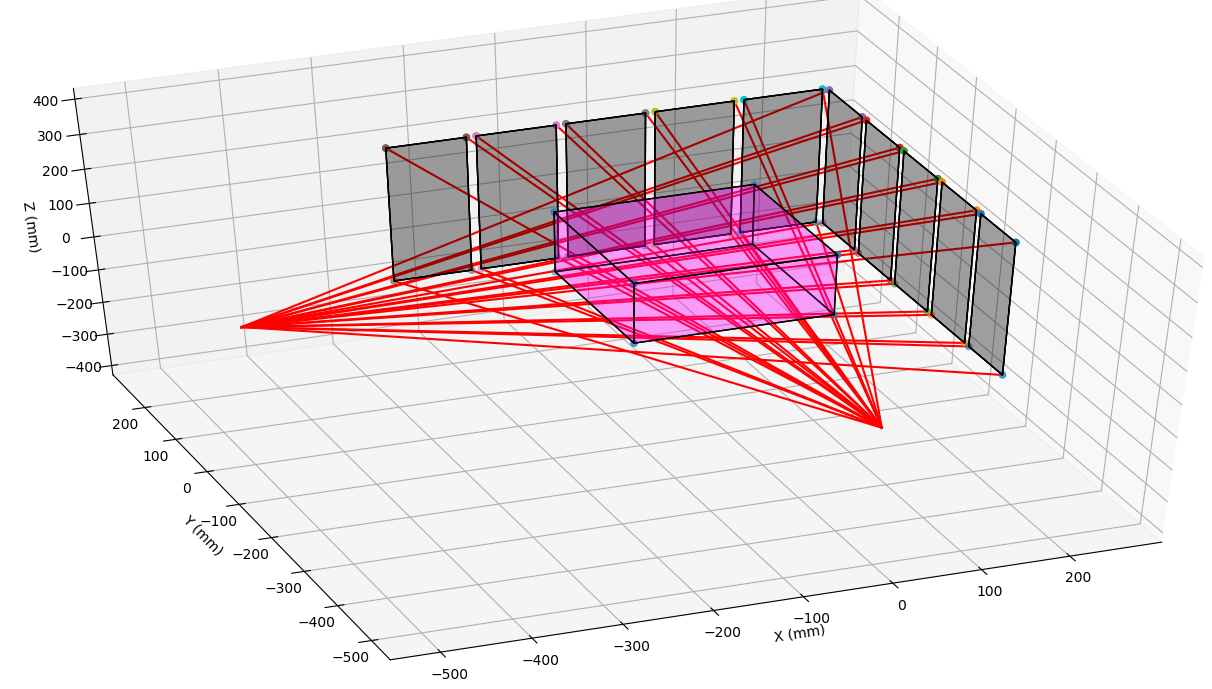
\includegraphics[scale=0.5]{modularBeam}
\end{center}
\caption{Sketch of a geometry built with the modular-beam framework.  The modules here lie on the perimeter of two sides of a rectangle as might exist for a carry-on luggage x-ray scanner.  This sketch was generated with the \texttt{sketch\_system()} Python function.  The  magenta box is the reconstruction volume, the gray rectangles are the detector panels, and the red lines trace from the source to each of the four corners of the detector.} \label{fig:modularBeamSketch}
\end{figure}
%\end{comment}

Now let $\bm{y}$ be a location of \texttt{sourcePositions}, $\bm{c}$ be a location of \texttt{moduleCenters}, $\bm{\widehat{v}}$ be a \texttt{rowVectors} instance, and $\bm{\widehat{u}}$ be a \texttt{colVectors} instance, and $D := \|\B{c}-\B{y}\|$. Then the X-ray Transform in modular-beam coordinate is given by
\begin{eqnarray*}
Pf(s,t) &:=& \int_{\mathbb{R}} f\left( \bm{y} + \frac{l}{\sqrt{D^2 + s^2 + t^2}}\left[ \bm{c}-\bm{y} + s\bm{\widehat{u}} + t\bm{\widehat{v}} \right] \right) \, dl.
\end{eqnarray*}


\section{Attenuated Radon Transform} \label{sec:ART}

The Attenuated Radon Transform (ART) and its adjoint in parallel-beam coordinates are given by
\begin{eqnarray*}
P_{\mu}f(s, \varphi, x_3) &=& \int_\mathbb{R} f(s\bm{\theta}^\perp(\varphi) - l\bm{\theta}(\varphi) + x_3\B{e}_3) e^{-\int_0^\infty \mu(s\bm{\theta}^\perp(\varphi) - (l+m)\bm{\theta}(\varphi)) \, dm} \, dl \\
P_{\mu}^*g(\bm{x}) &=& \int_0^{2\pi} g(\bm{x}\cdot\bm{\theta}^\perp(\varphi), \varphi, x_3) e^{-\int_0^\infty \mu(\B{x}-m\bm{\theta}(\varphi)) \, dm} \, d\varphi
\end{eqnarray*}
The object, f, can be reconstructed by the following Filtered Backprojection (FBP) algorithm
\begin{eqnarray*}
f(\bm{x}) &=& \frac{1}{4\pi} \text{Re div} \int_0^{2\pi} \bm{\theta}^\perp(\varphi) e^{\int_0^\infty \mu(\B{x}-m\bm{\theta}(\varphi)) \, dm} \left( e^{-h} H e^{h}g \right)(\bm{x}\cdot\bm{\theta}^\perp(\varphi), \varphi, x_3) \, d\varphi,
\end{eqnarray*}
where $h := \frac{1}{2}\left(I + iH\right) P\mu$, $I$ is the identify operator, and $H$ is the Hilbert Transform.

\section{Projectors for Cylindrically-Symmetric Objects}

The X-ray Transform for cylindrically-symmetric objects is the same as those X-ray Transforms for standard objects, but the volume is assumed to be cylindrically antisymmetric (the left and right sides can be different).  This object model causes the adjoint transform to take a very different form where there is a singularity along the axis of symmetry.  The FBP reconstruction algorithms are the same as those stated in the previous sections.  This is achieved by leveraging the fact that the object is symmetric and thus projections from all angles are the same.

\section{Anisotropic Total Variation}

LEAP has implementations of functions enabling anisotropic Total Variation (aTV) regularization.  The aTV functional is given by
\begin{eqnarray*}
R_\delta(f) &:=& \sum_i \sum_{j \in N(i)} \|i-j\| h_\delta(f_i-f_j),
\end{eqnarray*}
where $\|i-j\|$ is the distance between voxels $i$ and $j$, $N(i)$ is the neighborhood of voxel $i$ (in 3D, these are the 26 voxel neighbors), and $h_\delta$ is a Huber-like loss function given by
\begin{eqnarray*}
h_\delta(t) &:=& \begin{cases} \frac{1}{2}t^2, & |t| \leq \delta, \\ \frac{\delta^2}{6}\left[5\left|\frac{t}{\delta}\right|^{1.2}-2\right], & |t| > \delta \end{cases}.
\end{eqnarray*}
LEAP provides implementations of $R_\delta(f)$, $R_{\delta}'(f)$, and $<d, R_{\delta}''(f)d>$.  The inner product $<d, R_{\delta}''(f)d>$ is referred to as the \textit{quadratic form} of $R_\delta$ and is used to estimate the step size in gradient-based minimization algorithms of this functional.  The $\delta$ parameter is chosen by the user and should be approximately one-tenth of the difference between the two material types that one wishes to resolve.

\section{Matched Projector Models}

The projectors for parallel-, fan-, cone-, and axially aligned modular-beam geometries in LEAP are implemented by a method similar to the Separable Footprint (SF) method \cite{Long_TMI_2010}.  These projectors are matched, meaning that the backprojection operation is an exact transpose of the forward projection and they model the finite size of the voxel and detector pixels.  Our models are slightly faster than the original rectangle-rectangle SF method because they utilize the bilinear interpolation capabilities of texture memory, but are very, very slightly less accurate.

\section{Analytic Inversion Algorithms (FBP)} \label{sec:FBP}

LEAP contains an extensive collection of analytic inversion algorithms for parallel-, fan-, and cone-beam geometries with arbtirary detector shifts, offset center of rotation, non-equispaced projections angles, different angular ranges (short scan, full scan, over scan), axial or helical source trajectories, different voxels sizes and arbitary shifts of the volume location, etc.  Modular-beam geometries where the \texttt{rowVectors} are approximately equal to the positive z-axis can also be reconstruction with analytic inversion algorithms.  Inversion algorithms also exist for the Attenuated Radon Transform (ART) and objects with cylindrical symmetry (e.g., Abel Transform).  No matter the particular settings of any of these, the inversion algorithms in LEAP reconstruct quantitatively accurate volumes.  All of these algorithms are of Filtered Backprojection (FBP) type (e.g., FDK is an FBP type algorithm) algorithms and thus all one needs to do is specify the CT geometry and volume and then run the \texttt{FBP} command to perform the reconstruction.  No need to know what the actual algorithm is called.

With all that said there are a few LEAP parameters that perform some special case reconstructions.  Some of these are listed in table \ref{tab:FBPparameters}.  An example of one of these algorithms is the \textit{offsetScan} where the user deliberately offsets the detector and/or rotation stage to double the reconstructable field of view diameter with an FBP algorithm \cite{Gullberg_TMI_1986, Gregor_ICI_2003}.  This scanning strategy is also sometimes referred to as \textit{half-fan} or \textit{half-cone}.  A sketch of this idea is shown in Figure \ref{fig:offsetScan}.

\begin{table}[h!] \caption{Special purpose FBP parameters/algorithms} \label{tab:FBPparameters}
\begin{tabular}{l|p{11cm}}
function name & usage \\
\hline
\texttt{set\_offsetScan(bool)} & if set to true reconstructs data where the object extends past one side of the detector; can be used to double the diameter of the field of view, but requires projections over 360 degrees \\
\texttt{set\_truncatedScan(bool)} & if set to true will mitigate artifacts from object that extend past the right and left side of the detector (but does not increase the diameter of the field of view) \\
\texttt{set\_rampFilter(int)} & a larger number uses a sharper ramp filter; see Section \ref{sec:rampFilter}
\end{tabular}
\end{table}

\begin{figure}[h!]
\begin{tabular}{ccc}
\psset{unit=0.1mm}
\pspicture(-180,-50)(250,1000)%
% Detector
\psline[linewidth=2pt](-200,800)(200,800)
\psline[linestyle=dotted](0,0)(-200,800)
\psline[linestyle=dotted](0,0)(200,800)
\rput(0,830){detector}
% Source
\qdisk(0,0){2.5pt}
\rput(0,-30){source}
% source trajectory
\psarc[]{->}(0, 400){30}{0}{330}
% Field of View
\psarc[linecolor=red,linestyle=dashed](0, 400){100}{0}{360} % FOV
\rput(0,530){\red Field of View}
% center of rotation
\psset{linecolor=blue}
\qdisk(0,400){2.0pt}
\rput(0,300){\parbox{1.5cm}{\blue center of rotation}}
\psline{->}(0,340)(0,390)
\endpspicture
&
\psset{unit=0.1mm}
\pspicture(-250,-50)(250,1000)%
% Detector
\psline[linewidth=2pt](-200,800)(200,800)
\psline[linestyle=dotted](0,0)(-200,800)
\psline[linestyle=dotted](0,0)(200,800)
\rput(0,830){detector}
% Source
\qdisk(0,0){2.5pt}
\rput(0,-30){source}
% source trajectory
\psarc[]{->}(80, 400){30}{0}{330}
% Field of View
\psarc[linecolor=red,linestyle=dashed](80, 400){180}{0}{360} % FOV
\rput(80,600){\red Field of View}
% center of rotation
\psset{linecolor=blue}
\qdisk(80,400){2.0pt}
\rput(80,300){\parbox{1.5cm}{\blue center of rotation}}
\psline{->}(80,340)(80,390)
\endpspicture
&
\psset{unit=0.1mm}
\pspicture(-250,-50)(250,1000)%
% Detector
\psline[linewidth=2pt](-200,800)(200,800)
\psline[linestyle=dotted](150,0)(-200,800)
\psline[linestyle=dotted](150,0)(200,800)
\rput(0,830){detector}
% Source
\qdisk(150,0){2.5pt}
\rput(150,-30){source}
% source trajectory
\psarc[]{->}(160, 400){30}{0}{330}
% Field of View
\psarc[linecolor=red,linestyle=dashed](160, 400){175}{0}{360} % FOV
\rput(150,600){\red Field of View}
% center of rotation
\psset{linecolor=blue}
\qdisk(160,400){2.0pt}
\rput(160,300){\parbox{1.5cm}{\blue center of rotation}}
\psline{->}(160,340)(160,390)
\endpspicture
\end{tabular}
\caption{Increasing the imaging field of view with an \textit{offsetScan} FBP reconstruction. (left) Standard setup where the source, center of rotation, and detector are all centered. (middle) Offset scan setup where center of rotation is laterally translated.  This can be modeled in LEAP by shifting both the \texttt{tau} and \texttt{centerCol} parameters. (right) Offset scan (also can half-fan or half-cone) where the detector is laterally translated.  This can be modeled is LEAP by shfting the \texttt{centerCol} parameter.} \label{fig:offsetScan}
\end{figure}

\section{Digital Filters for CT}

Typical digital signal processing (DSP) texts are not motivated by imaging applications.  Many filters in these texts are designed for the one-dimensional DSP, such as the audio processing field and are ill-suited for imaging applications.  For example, many DSP texts state the superior interpolation performance of low-pass filters that approximate the \textit{ideal} low-pass filter (a rect function) over linear interpolation.  These approximations to the \textit{ideal} low-pass filter have sharp transitions in their frequency response which result in oscillatory impulse responses.  If used in imaging applications, these filters cause ringing artifacts (Gibb's phenomena) in the image and may also result in negative values in the filtered signal which may also be undesirable.  The sinc interpolation kernel of an \textit{ideal} low-pass filter is, in fact, just as arbitrary as any other interpolation kernel.  In some applications, a polynomial interpolation kernel will produce a more desired result.  Linear interpolation is computationally efficient, does not cause ringing artifacts, does not boost noise, produces a nonnegative output (provided that the input is nonnegative), is flexible, and easy to implement.

In this section we derive a collection of digital filters specifically designed for use in tomographic image reconstruction.  This includes the following filters: ramp, derivative, Hilbert, and low-pass.  We start with the ramp filter.

\subsection{Ramp Filter} \label{sec:rampFilter}

This section is focused on deriving discrete impulse responses for the ramp filter.  The (continous space) ramp filter for $f \in L^1(\mathbb{R}^n)$ is given by
\begin{eqnarray}
\R f(x) &:=& c_n \int_{\mathbb{R}^n} \frac{f(y)}{\| x-y\|^{n+1}} \, dy, \\
c_n &:=& -\frac{2}{(2\sqrt{\pi})^n} \frac{\Gamma(n)}{\Gamma(n/2)},
\end{eqnarray}
where $c_n = -\frac{1}{\pi}, -\frac{1}{2\pi}, -\frac{1}{\pi^2}$ for $n = 1, 2, 3$, respectively.  We also define the Fourier transform by
\begin{eqnarray}
\Fourier f(\xi) &:=& F(\xi) := \int_{\mathbb{R}^n} f(x) e^{-2\pi i <x,\xi>} \, dx.
\end{eqnarray}
Then $\Fourier \{\R f\}(\xi) = \|2\pi \xi\| F(\xi)$.

We define the Hilbert transform for $f \in L^1(\mathbb{R})$ by
\begin{eqnarray}
\Hilbert f(s) := \frac{1}{\pi}\int_\mathbb{R} \frac{f(t)}{s-t} \, dt.
\end{eqnarray}
With respect to Fourier transforms, the Hilbert transform is given by $$\Fourier \{\Hilbert f\}(\sigma) = i\sgn(\sigma)F(\sigma).$$  If we let $\mathcal{D} = \frac{d}{ds}$ be the derivative operator, then $\Fourier \{\mathcal{D} f\}(\sigma) = -2\pi i\sigma F(\sigma)$.  Therefore we have for $n = 1$ that $\R = \mathcal{D}\Hilbert = \Hilbert\mathcal{D}$.  We will exploit this property in the derivation of our discrete ramp filters.

Ramp filters are used in both analytic and iterative Computed Tomography (CT) image reconstruction algorithms.  The most common analytic CT image reconstruction algorithms are the filtered backprojection (FBP) and backprojection filtration (BPF) algorithms which require one and two dimensional ramp filters, respectively.  In iterative reconstruction one can use the 2D ramp filter as a preconditioner for the gradient descent or conjugate gradient algorithms to improve their rate of convergence.

The topic of digital ramp filter design has been addressed in a large amount of papers.  Most of these papers derive the digital impulse response by windowing the ideal ramp filter in frequency space.  Although this method of filter design allows the user to exactly specify the frequency response, the impulse response of many of these filters are highly oscillatory and thus produce results that are highly oscillatory which is undesirable.  For speed, application of the ramp filter is performed in the frequency domain using fast Fourier transform (FFT) operations, but all ramp filters are defined in the spatial domain to avoid a negative bias on the result \cite{Crawford_TMI_1991}.


\subsubsection{Derivation of Ramp Filters} \label{subset:rampFilterDevelopment}

The band-limited filter with least $L^2$ error is given by
\begin{eqnarray*}
h_{ramp}(s) &=& \int_{-1/2}^{1/2} 2\pi|\sigma| e^{2\pi i s\sigma} \, d\sigma \\
&=& 4\pi \int_0^{1/2} \sigma \cos(2\pi s \sigma) \, d\sigma \\
&=& \frac{\pi s\sin(\pi s) + \cos(\pi s) - 1}{\pi s^2}
\end{eqnarray*}
and the discrete filter is given by $h_{ramp}[k] = h_{ramp}(k) = \frac{(-1)^k-1}{\pi k^2}$.  This is known as the Ram-Lak filter and thus we define $h_{RL}[k] := h_{ramp}[k]$.  Although the frequency response of this filter is ideal, the impulse response oscillates with every sample as shown in Figure \ref{fig:impulseResponse}.  Thus we see that convolution with this filter will invariably produce oscillatory functions which is undesired.  To understand and mitigate this effect we focus on the Hilbert transform which is one part of the ramp filter.  

Now the band-limited Hilbert filter is given by
\begin{eqnarray}
h_{hilb}(s) &:=& \int_{-1/2}^{1/2} i\sgn(\sigma) e^{2\pi i s \sigma} \, d\sigma \\
&=& \frac{1-\cos(\pi s)}{\pi s}.
\end{eqnarray}
Note that $h_{hilb}'(s) = h_{ramp}(s)$, as expected. Now consider two discrete Hilbert filters
\begin{eqnarray}
h_{hilb}[k] &:=& h_{hilb}(k) = \frac{1 - (-1)^k}{\pi k} \\
h_{hilb,1/2}[k] &:=& h_{hilb}(k-1/2) = \frac{1}{\pi(k-\frac{1}{2})}. \label{eq:shiftedHilbertFilter}
\end{eqnarray}
In Figure \ref{fig:HilbertImpulseResponse} we notice that while $h_{hilb}[k]$ is oscillatory, $h_{hilb,1/2}[k]$ is not.  This oscillatory behavior can thus be removed by introduceing a (backward) half sample shift into the filter.  Now we can define a ramp filter by convolving $h_{hilb,1/2}[k]$ with a finite difference filter with a half sample forward shift.

\begin{figure}[h]
\begin{center}
\psset{xunit=0.4cm,yunit=5.0cm}
\begin{pspicture}(-20,-0.7)(20,0.7)
\psaxes[ticks=none,labels=none,linewidth=0.5pt,linestyle=dashed]{<->}(0,0)(-21,-0.8)(21,0.8)
%\psplot[plotpoints=41,linewidth=1.25pt,linecolor=blue,showpoints=true]{-20}{20}{1 x 0.5 sub div 0.3183098861837907 mul}
\psplot[plotpoints=21,linewidth=1.25pt,linecolor=blue,showpoints=true]{-20.5}{-0.5}{1 x div 0.3183098861837907 mul}
\psplot[plotpoints=20,linewidth=1.25pt,linecolor=blue,showpoints=true]{0.5}{19.5}{1 x div 0.3183098861837907 mul}
\psline[linewidth=1.25pt,linecolor=blue](-0.5,-0.63661977236758133307)(0.5,0.63661977236758133307)
\psplot[plotpoints=20,linewidth=1.25pt,linecolor=red,showpoints=true]{-20}{-1}{1 -1 x exp sub x div 0.3183098861837907 mul}
\psplot[plotpoints=20,linewidth=1.25pt,linecolor=red,showpoints=true]{1}{20}{1 -1 x exp sub x div 0.3183098861837907 mul}
\psline[linewidth=1.25pt,linecolor=red](-1,-0.63661977236758133307)(0,0)(1,0.63661977236758133307)
\psplot{-20}{-0.01}{1 180 x mul cos sub x div 0.3183098861837907 mul}
\psplot{0.01}{20}{1 180 x mul cos sub x div 0.3183098861837907 mul}
\end{pspicture}
\end{center}
\caption{Discrete impulse response of the ideal Hilbert filter with zero shift (red) and half shift (blue).  The continuous space impulse response is shown in black.} \label{fig:HilbertImpulseResponse}
\end{figure}

We find the finite difference coefficients by solving the following linear system
\begin{eqnarray}
\begin{bmatrix} 2 \\ 0 \\ 0 \\ \vdots \\ 0 \end{bmatrix} &=& \begin{bmatrix} 1 & 3 & 5 & \cdots & 2M-1 \\ 1 & 3^3 & 5^3 & \cdots & (2M-1)^3 \\ 1 & 3^5 & 5^5 & \cdots & (2M-1)^5 \\ \vdots & \vdots & \vdots & \ddots & \vdots \\ 1 & 3^{2M-1} & 5^{2M-1} & \cdots & (2M-1)^{2M-1} \end{bmatrix} \begin{bmatrix} a_0 \\ a_1 \\ a_2 \\ \vdots \\ a_{M-1} \end{bmatrix} \label{eq:derivEq1} \\
h_{d,2M}[k] &:=& \frac{1}{2}\begin{cases} -a_{-k}, & k = -M+1, -M+2, \dots 0, \\ a_{k-1}, & k = 1, 2, \dots, M \end{cases} \label{eq:derivEq2}
\end{eqnarray}
and thus for $M = 1, 2, 3, 4, 5$ the filter coefficients are given by
\begin{eqnarray}
\{h_{d,2}[k]\}_{k=0}^1 &:=& \left\{-1, 1\right\} \label{eq:DERIV_FD2} \\
\{h_{d,4}[k]\}_{k=-1}^2 &:=& \left\{\frac{1}{24}, -\frac{9}{8}, \frac{9}{8}, -\frac{1}{24}\right\} \label{eq:DERIV_FD4} \\
\{h_{d,6}[k]\}_{k=-2}^3 &:=& \left\{-\frac{3}{640}, \frac{25}{384}, -\frac{75}{64}, \frac{75}{64}, -\frac{25}{384}, \frac{3}{640}\right\} \label{eq:DERIV_FD6} \\
\{h_{d,8}[k]\}_{k=-3}^4 &:=& \left\{\frac{5}{7168}, -\frac{49}{5120}, \frac{245}{3072}, -\frac{1225}{1024}, \frac{1225}{1024}, -\frac{245}{3072}, \frac{49}{5120}, -\frac{5}{7168}\right\}  \label{eq:DERIV_FD8} \\
\{h_{d,10}[k]\}_{k=-4}^5 &:=& \left\{-\frac{35}{294912}, \frac{405}{229376}, -\frac{567}{40960}, \frac{735}{8192}, -\frac{19845}{16384}, \right. \notag \\ && \left. \quad \; \; \frac{19845}{16384}, -\frac{735}{8192}, \frac{567}{40960}, -\frac{405}{229376}, \frac{35}{294912} \right\} \label{eq:DERIV_FD10}
\end{eqnarray}
Note that $h_{d,M}$ has $M$ nonzero entries and is accurate to the $M$th order, i.e., $f'\left(\frac{1}{2}T\right) = f(kT) * h_{d,M}[k] + O(T^M)$ as $T \ra 0$.  The impulse response of the limiting case is given by
\begin{eqnarray}
h_{d,\infty}[k] &:=& \lim_{M \ra \infty} h_{d,M}[k] = \frac{(-1)^k}{\pi\left(k+\frac{1}{2}\right)^2}.
\end{eqnarray}

The impulse response of the M-th order digital ramp filter is given by
\begin{eqnarray}
h_M[k] := h_{hilb,1/2} * h_{d,M}[k], \label{eq:convHilbertAndDeriv}
\end{eqnarray}
where
\begin{eqnarray}
h_2[k] &:=& \frac{1}{\pi\left(\frac{1}{4}-k^2\right)} \label{eq:RAMP_FD2} \\
h_4[k] &:=& \frac{1}{\pi\left(\frac{1}{4}-k^2\right)} \frac{k^2-\frac{5}{2}}{k^2-\frac{9}{4}} \label{eq:RAMP_FD4} \\
h_6[k] &:=& \frac{1}{\pi\left(\frac{1}{4}-k^2\right)} \frac{k^4-\frac{35}{4}k^2+\frac{259}{16}}{\left(k^2-\frac{9}{4}\right)\left(k^2-\frac{25}{4}\right)} \label{eq:RAMP_FD6} \\
h_8[k] &:=& \frac{1}{\pi\left(\frac{1}{4}-k^2\right)} \frac{k^6-\frac{336}{16}k^4+\frac{1974}{16}k^2-\frac{3229}{16}}{\left(k^2-\frac{9}{4}\right)\left(k^2-\frac{25}{4}\right)\left(k^2-\frac{49}{4}\right)} \label{eq:RAMP_FD8} \\
h_{10}[k] &:=& \frac{1}{\pi\left(\frac{1}{4}-k^2\right)} \frac{k^8 - \frac{165}{4}k^6 + \frac{4389}{8}k^4 - \frac{86405}{32}k^2 + \frac{1057221}{256}}{\left(k^2-\frac{9}{4}\right)\left(k^2-\frac{25}{4}\right)\left(k^2-\frac{49}{4}\right)\left(k^2-\frac{81}{4}\right)} \label{eq:RAMP_FD10}
\end{eqnarray}
and the corresponding frequency responses are given by
\begin{eqnarray}
H_2(X) &:=& \left[2\sin\left(\pi X\right)\right]\sgn(X) \label{eq:rampFreq2} \\
H_4(X) &:=& \left[\frac{9}{4}\sin\left(\pi X\right) - \frac{1}{12}\sin\left(3\pi X\right)\right]\sgn(X) \\
H_6(X) &:=& \left[\frac{75}{32}\sin\left(\pi X\right) - \frac{25}{192}\sin\left(3\pi X\right) + \frac{3}{320}\sin\left(5\pi X\right)\right]\sgn(X) \\
H_8(X) &:=& \left[\frac{1225}{512}\sin\left(\pi X\right) - \frac{245}{1536}\sin\left(3\pi X\right) \right. \notag \\ &+& \left. \frac{49}{2560}\sin\left(5\pi X\right) - \frac{5}{3584}\sin\left(7\pi X\right)\right]\sgn(X) \\
H_{10}(X) &:=& \left[\frac{19845}{8192}\sin\left(\pi X\right) - \frac{735}{4096}\sin\left(3\pi X\right) + \frac{567}{20480}\sin\left(5\pi X\right) \right. \notag \\ &-& \left. \frac{405}{114688}\sin\left(7\pi X\right) + \frac{35}{147456}\sin\left(9\pi X\right)\right]\sgn(X) \label{eq:rampFreq10}
\end{eqnarray}
for $X \in \left[-\frac{1}{2}, \frac{1}{2}\right)$.  The impulse and frequency responses of these filters are shown in Figures \ref{fig:impulseResponse} and \ref{fig:frequencyResponse}, respectively.  Note that $h_{\infty}[k] = h_{RL}[k]$.

We additionally define $h_0[k] := h_2[k] * \left\{ \frac{1}{4}, \frac{1}{2}, \frac{1}{4} \right\} = h_2[k] \frac{k^2-\frac{3}{4}}{k^2-\frac{9}{4}}$ and $H_0(X) = H_2(X)\frac{1+\cos(2\pi X)}{2}$.  The zero subscript here does not specify the order of the finite difference as in the other filter definitions, but was chosen to uniformity of notation and to denote that the frequency response of this filter at Nyquist is zero.

Note that the sign of the derivative of these filters only changes three times, while the sign of the derivative of $h_{RL}[n]$ changes with every sample.

Since $h_M[k]$ have infinite impulse response (IIR), one must window these filters.  Suppose one wishes to filter $g[k]$, where $g[k] \neq 0$ for $k = -N/2, \dots, N/2-1$ with the ramp filter.  Then one can filter the data using FFT operations by
\begin{eqnarray*}
IFFT_{2N}(FFT_{2N}(g) FFT_{2N}(w h_M))[k],
\end{eqnarray*}
where $w[k]$ is a window function ($w[k] = 0$ for $k \notin [-N, N-1]$) and $FFT_{2N}$ and $IFFT_{2N}$ are the $2N$ point Fast Fourier Transform and Inverse Fast Fourier Transform operations, respectively.  Since $h_M[k] = O(k^{-2})$, the ramp filter decays rapidly and thus one can use the rectangular window given by $$w[k] = \begin{cases} 1, & k = -N, -N+1, \dots, N-1, \\ 0, & \text{otherwise} \end{cases}$$ without any significant distortion of the frequency response.  It is advised that one performs the filtering in this fashion, rather than using equations (\ref{eq:rampFreq2}-\ref{eq:rampFreq10}) explicitly.

\begin{figure}[h]
\begin{center}
\psset{xunit=0.75cm,yunit=3.75cm}
\begin{pspicture}(-10,-0.45)(10,1.75)
\psaxes[ticks=none,labels=none,linewidth=0.5pt,linestyle=dashed]{<->}(0,0)(-11,-0.6)(11,1.7)
\psplot[plotpoints=21,linewidth=1.25pt,showpoints=true]{-10}{10}{1 0.25 x x mul sub div 0.3183098861837907 mul}
\psplot[plotpoints=21,linewidth=1.25pt,showpoints=true,linecolor=blue]{-10}{10}{1 0.25 x x mul sub div 2.5 x x mul sub 2.25 x x mul sub div mul 0.3183098861837907 mul}
\psplot[plotpoints=10,linewidth=1.25pt,showpoints=true,linecolor=red]{-10}{-1}{-1 x exp 1 sub x x mul div 0.3183098861837907 mul}
\psplot[plotpoints=10,linewidth=1.25pt,showpoints=true,linecolor=red]{1}{10}{-1 x exp 1 sub x x mul div 0.3183098861837907 mul}
\psline[linewidth=1.25pt,showpoints=true,linecolor=red](-1,-0.63661977236758133307)(0,1.5707963267948966613)(1,-0.63661977236758133307)
\end{pspicture}
\end{center}
\caption{Impulse response of Ram-Lak (red), $h_4[k]$ (blue), and $h_2[k]$ (Shepp-Logan, black) ramp filters.} \label{fig:impulseResponse}
\end{figure}

% pi/2 = 1.57079632679489658
% pi   = 3.14159265358979311
% 1/12 = 0.08333333333333333
\begin{figure}[h]
\begin{center}
\psset{xunit=10.0cm,yunit=1.8cm}
\begin{pspicture}(-0.5,-0.05)(0.5,3.2)
\psaxes[ticks=none,labels=none,linewidth=0.5pt]{<->}(0,0)(-0.55,0)(0.55,3.3)
\psline(-0.05,3.14159265358979311)(0.05,3.14159265358979311) \rput(0.075,3.14159265358979311){\Large $\pi$}
\psline(0.5,-0.1)(0.5,0.1) \rput(0.485,-0.25){\Large $\frac{1}{2}$} \psline(-0.5,-0.1)(-0.5,0.1) \rput(-0.485,-0.25){\Large $-\frac{1}{2}$}
%\psplot[linecolor=black]{0}{0.5}{180 x mul sin 2 mul 0.5 0.5 360 x mul cos mul add mul}
%\psplot[linecolor=black]{-0.5}{0}{-1 180 x mul sin 2 mul 0.5 0.5 360 x mul cos mul add mul mul}

%\psplot[linecolor=black]{0}{0.5}{180 x mul sin 2 mul 5 8 div 0.5 360 x mul cos mul add -0.125 720 x mul cos mul add mul}
%\psplot[linecolor=black]{-0.5}{0}{-1 180 x mul sin 2 mul 5 8 div 0.5 360 x mul cos mul add -0.125 720 x mul cos mul add mul mul}

%\psplot[linecolor=black]{0}{0.5}{180 x mul sin 2 mul 0.6875 0.4688 360 x mul cos mul add -0.1875 720 x mul cos mul add 0.0313 1080 x mul cos mul add mul}
%\psplot[linecolor=black]{-0.5}{0}{-1 180 x mul sin 2 mul 0.6875 0.4688 360 x mul cos mul add -0.1875 720 x mul cos mul add 0.0313 1080 x mul cos mul add mul mul}

\psplot[linecolor=black]{0}{0.5}{180 x mul sin 2 mul} \psplot[linecolor=black]{-0.5}{0}{180 x mul sin -2 mul}
\psplot[linecolor=blue]{0}{0.5}{180 x mul sin 2.25 mul 540 x mul sin -0.08333333333333333 mul add} \psplot[linecolor=blue]{-0.5}{0}{180 x mul sin -2.25 mul 540 x mul sin 0.08333333333333333 mul add}
\psplot[linecolor=cyan]{0}{0.5}{360 2 div x mul sin 75 32 div mul 3 360 2 div mul x mul sin -25 192 div mul add 5 360 2 div mul x mul sin 3 320 div mul add}
\psplot[linecolor=cyan]{-0.5}{0}{-1 360 2 div x mul sin 75 32 div mul 3 360 2 div mul x mul sin -25 192 div mul add 5 360 2 div mul x mul sin 3 320 div mul add mul}
\psplot[linecolor=magenta]{0}{0.5}{360 2 div x mul sin 1225 512 div mul 3 360 2 div mul x mul sin -245 1536 div mul add 5 360 2 div mul x mul sin 49 2560 div mul add 7 360 2 div mul x mul sin -5 3584 div mul add}
\psplot[linecolor=magenta]{-0.5}{0}{-1 360 2 div x mul sin 1225 512 div mul 3 360 2 div mul x mul sin -245 1536 div mul add 5 360 2 div mul x mul sin 49 2560 div mul add 7 360 2 div mul x mul sin -5 3584 div mul add mul}
\psplot[linecolor=green]{0}{0.5}{2 360 2 div x mul sin 19845 16384 div mul 3 360 2 div mul x mul sin -735 8192 div mul add 5 360 2 div mul x mul sin 567 40960 div mul add 7 360 2 div mul x mul sin -405 229376 div mul add 9 360 2 div mul x mul sin 35 294912 div mul add mul}
\psplot[linecolor=green]{-0.5}{0}{-2 360 2 div x mul sin 19845 16384 div mul 3 360 2 div mul x mul sin -735 8192 div mul add 5 360 2 div mul x mul sin 567 40960 div mul add 7 360 2 div mul x mul sin -405 229376 div mul add 9 360 2 div mul x mul sin 35 294912 div mul add mul}
\psplot[linecolor=red]{0}{0.5}{3.14159265358979311 2 mul x mul} \psplot[linecolor=red]{-0.5}{0}{-3.14159265358979311 2 mul x mul} % 2pi x
\rput[r](-0.5,3.14){\red $H_{RL}(X)$}
\rput[l](0.5,2.6334){\green $H_{10}(X)$}
\rput[r](-0.5,2.56){\magenta $H_8(X)$}
\rput[l](0.5,2.46){\cyan $H_6(X)$}
\rput[r](-0.5,2.3){\blue $H_4(X)$}
\rput[l](0.5,1.975){\black $H_2(X)$}
\end{pspicture}
\end{center}
\caption{Frequency response of Ram-Lak (red), $H_{10}(X)$ (green), $H_8(X)$ (magenta), $H_6(X)$ (cyan), $H_4(X)$ (blue), and $H_2(X)$ (Shepp-Logan, black) ramp filters.} \label{fig:frequencyResponse}
\end{figure}

\begin{table}[h]
\caption{Relative $L^2$ difference $\left( \frac{\| H_M - H_{RL} \|}{\| H_{RL} \|} \right)$ between $H_M(X)$ and $H_{RL}(X)$.}
\begin{center}
\begin{tabular}{l|l}
Filter & Relative $L^2$ Difference \\
\hline
$H_2(X)$ & 24.5\% \\ % 77.97\% = sqrt(sumAll(h_M.^2)/sumAll(h_RL.^2))*100
$H_4(X)$ & 14.7\% \\ % 87.78\%
$H_6(X)$ & 10.9\% \\ % 91.51\%
$H_8(X)$ & 8.7\% \\ % 93.48\%
$H_{10}(X)$ & 7.4\% % 94.71\%
\end{tabular}
\end{center}
\end{table}

Higher order filters can be found using equations (\ref{eq:shiftedHilbertFilter}, \ref{eq:derivEq1}, \ref{eq:derivEq2}, \ref{eq:convHilbertAndDeriv}), but are unlikely to provide more accurate reconstructions because they will further amplify noise and ringing artifacts and some of the gained resolution will be lost in the interpolation methods used in the backproject step of FBP or BPF.

\subsubsection{Two Dimensional Extensions}

The filters defined above can be extended to two dimensions by the following
\begin{eqnarray}
H_{2D}(X,Y) &:=& \sqrt{H^2(X) + H^2(Y) - \frac{1}{H^2(1/2)}H^2(X)H^2(Y)}.
\end{eqnarray}
Note that $H_{2D}(X,0) = H(X)$, $H_{2D}(0,Y) = H(Y)$, and $H_{2D}(X,\pm 1/2) = H_{2D}(\pm 1/2, Y) = H(1/2)$.  Thus we see that $H_{2D}(X,Y)$ (including its periodic extension) is infinitely differentiable everywhere except at the origin.  This ensures that the impulse response will decay rapidly.

One can show and it is well known that $\mathcal{R} = -\Delta$, where $\Delta = \sum_i \frac{\partial^2}{\partial x_i^2}$ is the Laplace operator.  Using $H(X) = H_2(X)$, we have that
\begin{eqnarray*}
H_{2D}^2(X,Y) = 4\sin^2(\pi X) + 4\sin^2(\pi Y) - 4\sin^2(\pi X)\sin^2(\pi Y)
\end{eqnarray*}
which is the frequency response of $$-\begin{bmatrix} 0.25 & 0.5 & 0.25 \\ 0.5 & -3 & 0.5 \\ 0.25 & 0.5 & 0.25 \end{bmatrix}.$$  This is a common filter for the discrete Laplacian, where the weight of the derivative on the diagonals are weighted by their distance from the center sample.  Thus we see that our choice of $H_{2D}(X,Y)$ is not only practical, but also theoretically relevant.

It is sometimes advantageous to add a lowpass filter, $U(X)$, to the ramp filter by $H_{LP}(X) := U(X)H(X)$, where $U(0) = 1$ and $U(\pm 1/2) = 0$.  One can extend this to the 2D ramp filter by
\begin{eqnarray}
H_{2D,LP}(X,Y) &:=& U(X)U(Y)\sqrt{H^2(X) + H^2(Y) - \frac{1}{H^2(1/2)}H^2(X)H^2(Y)}.
\end{eqnarray}

\subsubsection{Edge Response and Modular Transfer Functions}

We illustrate the resolution of the filters defined above by performing a simulation experiment.  We simulated a circular disk and reconstructed it with a collection of filters.  The edge spread function (ESF) and modular transfer function (MTF) plots are shown in Figure \ref{fig:ESF_MTF}.  We also include a common ramp filter, which we denote $h_{Butterworth}[k]$ and is given by $H_{Butterworth}(X) = H_{RL}(X) \frac{1}{1+X^{10}}$.  Note that the ESF of $h_{Butterworth}[k]$ is highly oscillatory (even more so than the Ram-Lak filter).  The filter $h_4[k]$ has nearly identical resolution as $h_{Butterworth}[k]$, but with very little ringing.

\begin{figure}[h]
\begin{tabular}{ccc}
\includegraphics[scale=0.3]{ESF}
& \includegraphics[scale=0.3]{ESF_zoom}
& \includegraphics[scale=0.3]{MTF}
\end{tabular}
\caption{The ESF and MTF using $h_0[k]$, $h_2[k]$, $h_4[k]$, $h_{10}[k]$, $h_{RL}[k]$, and $h_{Butterworth}[k]$.} \label{fig:ESF_MTF}
\end{figure}


% BIBLIOGRAPHY
\begin{thebibliography}{100}

\bibitem{DeManBasu_PMB_2004} De Man, Bruno, and Samit Basu. ``Distance-driven projection and backprojection in three dimensions.'' \emph{Physics in Medicine \& Biology} 49, no. 11 (2004): 2463.

\bibitem{ChampleyLTT} Champley, Kyle M., Trevor M. Willey, Hyojin Kim, Karina Bond, Steven M. Glenn, Jerel A. Smith, Jeffrey S. Kallman et al. ``Livermore tomography tools: Accurate, fast, and flexible software for tomographic science.'' \emph{NDT \& E International} 126 (2022): 102595.

\bibitem{Long_TMI_2010} Long, Yong, Jeffrey A. Fessler, and James M. Balter. ``3D forward and back-projection for X-ray CT using separable footprints.'' \emph{IEEE transactions on medical imaging} 29, no. 11 (2010): 1839-1850.

\bibitem{ChampleyMaddox_Optica_2021} Champley, Kyle, and Brian Maddox. ``Model based iterative reconstruction with the tilted Abel Transform.'' \emph{In Digital Holography and Three-Dimensional Imaging}, pp. DF4F-1. Optica Publishing Group, 2021.

\bibitem{ASDPOCS_PMB_2008} Sidky, Emil Y., and Xiaochuan Pan. ``Image reconstruction in circular cone-beam computed tomography by constrained, total-variation minimization.'' \emph{Physics in Medicine \& Biology} 53, no. 17 (2008): 4777.

\bibitem{Hager_Zhang_CG_2005} William W. Hager and Hongchao Zhang, ``A Survey of Nonlinear Conjugate Gradient Methods,'' \emph{AMS}, 2005

\bibitem{Fessler_TIP_1999}Jeffrey A. Fessler and Scott D. Booth. ``Conjugate-gradient preconditioning methods for shift-variant pet image reconstruction,'' \emph{IEEE Trans. Imag. Proc.}, Vol. 8, pp. 688-699, 1999

\bibitem{Yu_MIC_2006} Zhou Yu, Jean-Baptiste Thibault, Ken Sauer, Charles Bouman, and Jiang Hsieh, ``Accelerated Line Search for Coordinate Descent
Optimization,'' \emph{IEEE Nuclear Science Symposium Conference Record}, 2006

\bibitem{IMPACT_TMI_2001} De Man, Bruno, Johan Nuyts, Patrick Dupont, Guy Marchal, and Paul Suetens. ``An iterative maximum-likelihood polychromatic algorithm for CT.'' IEEE transactions on medical imaging 20, no. 10 (2001): 999-1008.

\bibitem{Joseph_TMI_1982} Joseph, Peter M. ``An improved algorithm for reprojecting rays through pixel images.'' \emph{IEEE transactions on medical imaging} 1, no. 3 (1982): 192-196.

\bibitem{Parker_MP_1982} D. L. Parker, ``Optimal short scan convolution reconstruction for fan-beam CT,'' \emph{Medical Physics}, 9:254–257, 
1982

\bibitem{Natterer_IP_2001} Frank Natterer, ``Inversion of the attenuated radon transform'', \emph{Inverse Problems} 17 (2001), 113–119

\bibitem{FDK} Feldkamp, Lee A., Lloyd C. Davis, and James W. Kress. ``Practical cone-beam algorithm.'' Josa a 1, no. 6 (1984): 612-619.

\bibitem{Katsevich_SIAM_2002} Katsevich, Alexander. ``Theoretically exact filtered backprojection-type inversion algorithm for spiral CT.'' SIAM Journal on Applied Mathematics 62, no. 6 (2002): 2012-2026.

\bibitem{WFBP} Stierstorfer, Karl, Annabella Rauscher, Jan Boese, Herbert Bruder, Stefan Schaller, and Thomas Flohr. ``Weighted FBP—a simple approximate 3D FBP algorithm for multislice spiral CT with good dose usage for arbitrary pitch.'' Physics in Medicine \& Biology 49, no. 11 (2004): 2209.

\bibitem{NHDLH_PMB_2007} Noo, Frederic, Stefan Hoppe, Frank Dennerlein, Günter Lauritsch, and Joachim Hornegger. ``A new scheme for view-dependent data differentiation in fan-beam and cone-beam computed tomography.'' Physics in Medicine \& Biology 52, no. 17 (2007): 5393.

\bibitem{Gullberg_TMI_1986} Gullberg, Grant T., Carl R. Crawford, and Benjamin MW Tsui. ``Reconstruction algorithm for fan beam with a displaced center-of-rotation.'' IEEE transactions on medical imaging 5, no. 1 (1986): 23-29.

\bibitem{Gregor_ICI_2003} Gregor, Jens, Shaun S. Gleason, and Michael J. Paulus. ``Conebeam x-ray computed tomography with an offset detector array.'' In Proceedings 2003 International Conference on Image Processing (Cat. No. 03CH37429), vol. 2, pp. II-803. IEEE, 2003.

\bibitem{Crawford_TMI_1991} Crawford, Carl R. ``CT filtration aliasing artifacts.'' IEEE transactions on medical imaging 10, no. 1 (1991): 99-102.

\end{thebibliography}
\end{document}
